

%%
%% This is file `sample-sigconf.tex',
%% generated with the docstrip utility.
%%
%% The original source files were:
%%
%% samples.dtx  (with options: `all,proceedings,bibtex,sigconf')
%% 
%% IMPORTANT NOTICE:
%% 
%% For the copyright see the source file.
%% 
%% Any modified versions of this file must be renamed
%% with new filenames distinct from sample-sigconf.tex.
%% 
%% For distribution of the original source see the terms
%% for copying and modification in the file samples.dtx.
%% 
%% This generated file may be distributed as long as the
%% original source files, as listed above, are part of the
%% same distribution. (The sources need not necessarily be
%% in the same archive or directory.)
%%
%%
%% Commands for TeXCount
%TC:macro \cite [option:text,text]
%TC:macro \citep [option:text,text]
%TC:macro \citet [option:text,text]
%TC:envir table 0 1
%TC:envir table* 0 1
%TC:envir tabular [ignore] word
%TC:envir displaymath 0 word
%TC:envir math 0 word
%TC:envir comment 0 0
%%
%% The first command in your LaTeX source must be the \documentclass
%% command.
%%
%% For submission and review of your manuscript please change the
%% command to \documentclass[manuscript, screen, review]{acmart}.
%%
%% When submitting camera ready or to TAPS, please change the command
%% to \documentclass[sigconf]{acmart} or whichever template is required
%% for your publication.
%%
%%
\documentclass[sigconf]{acmart}
% \settopmatter{printacmref=false}
% \settopmatter{printccs=false}
% \settopmatter{printkeywords=false}

\usepackage{makecell}
\usepackage{subcaption}
% \usepackage{subcaption}

% \usepackage[T1]{fontenc}
% \usepackage[utf8]{inputenc}
% \usepackage{amsmath, amssymb, amsfonts}
% \usepackage{graphicx, float}
% \usepackage[hidelinks]{hyperref}
\usepackage{algorithm}
% % \usepackage{algorithmic}
% \usepackage{tikz}
% \usepackage{xcolor}
\newcommand{\edited}[1]{#1}
% \usepackage{soul}
% \sethlcolor{yellow}
% \usepackage{makecell}
% \usepackage{booktabs} 
% \newcommand{\highlight}[1]{\hl{#1}}
% \newcommand{\name}{{{\tt UWB-IVPL}}}

% \usetikzlibrary{arrows.meta, bending, positioning}
% \usepackage{csquotes}
% \usepackage[english]{babel}
% \usepackage[style=ieee]{biblatex}
% \usepackage{biblatex}
% \addbibresource{references.bib}
%%
%% \BibTeX command to typeset BibTeX logo in the docs
\AtBeginDocument{%
  \providecommand\BibTeX{{%
    Bib\TeX}}}

%% Rights management information.  This information is sent to you
%% when you complete the rights form.  These commands have SAMPLE
%% values in them; it is your responsibility as an author to replace
%% the commands and values with those provided to you when you
%% complete the rights form.
% \setcopyright{acmlicensed}
% \copyrightyear{2018}
% \acmYear{2018}
% \acmDOI{XXXXXXX.XXXXXXX}
% %% These commands are for a PROCEEDINGS abstract or paper.
% \acmConference[SenSys '26]{International Conference on Embedded Artificial Intelligence and Sensing Systems}{May 11-14, 2026}{Saint-Malo, France}

% %%
% %%  Uncomment \acmBooktitle if the title of the proceedings is different
% %%  from ``Proceedings of ...''!
% %%
% %%\acmBooktitle{Woodstock '18: ACM Symposium on Neural Gaze Detection,
% %%  June 03--05, 2018, Woodstock, NY}
% \acmISBN{978-1-4503-XXXX-X/2018/06}

\copyrightyear{2026}
\acmYear{2026}
\setcopyright{cc}
\setcctype{by}
\acmConference[SenSys '26]{ACM/IEEE International Conference on Embedded Artificial Intelligence and Sensing Systems}{May 11--14, 2026}{Saint Malo, France}
\acmBooktitle{ACM/IEEE International Conference on Embedded Artificial Intelligence and Sensing Systems (SenSys '26), May 11--14, 2026, Saint Malo, France}
\acmDOI{10.1145/3774906.3800472}
\acmISBN{979-8-4007-2309-4/2026/05}
\newcommand{\name}{{{\tt UWB-PTrac}}}
\newcommand{\vp}{\vspace{-1.5em}}

%%
%% Submission ID.
%% Use this when submitting an article to a sponsored event. You'll
%% receive a unique submission ID from the organizers
%% of the event, and this ID should be used as the parameter to this command.
%%\acmSubmissionID{123-A56-BU3}

%%
%% For managing citations, it is recommended to use bibliography
%% files in BibTeX format.
%%
%% You can then either use BibTeX with the ACM-Reference-Format style,
%% or BibLaTeX with the acmnumeric or acmauthoryear sytles, that include
%% support for advanced citation of software artefact from the
%% biblatex-software package, also separately available on CTAN.
%%
%% Look at the sample-*-biblatex.tex files for templates showcasing
%% the biblatex styles.
%%

%%
%% The majority of ACM publications use numbered citations and
%% references.  The command \citestyle{authoryear} switches to the
%% "author year" style.
%%
%% If you are preparing content for an event
%% sponsored by ACM SIGGRAPH, you must use the "author year" style of
%% citations and references.
%% Uncommenting
%% the next command will enable that style.
%%\citestyle{acmauthoryear}


%%
%% end of the preamble, start of the body of the document source.
\pagestyle{plain}
\begin{document}

%%
%% The "title" command has an optional parameter,
%% allowing the author to define a "short title" to be used in page headers.
\title{UWB-Based Localization of Smartphones Inside a Vehicle to Prevent Distracted Driving}


%%
%% The "author" command and its associated commands are used to define
%% the authors and their affiliations.
%% Of note is the shared affiliation of the first two authors, and the
%% "authornote" and "authornotemark" commands
%% used to denote shared contribution to the research.
% \author{Ben Trovato}
% \authornote{Both authors contributed equally to this research.}
% \email{trovato@corporation.com}
% \orcid{1234-5678-9012}
% \author{G.K.M. Tobin}
% \authornotemark[1]
% \email{webmaster@marysville-ohio.com}
% \affiliation{%
%   \institution{Institute for Clarity in Documentation}
%   \city{Dublin}
%   \state{Ohio}
%   \country{USA}
% }
% \author{Paper \#112}
\author{Kailai Cui}
\affiliation{%
  \institution{University Of Michigan - Ann Arbor}
  \city{Ann Arbor}
   \state{MI}
  \country{USA}}
\email{kailaic@umich.edu}

\author{Ke Sun}
\affiliation{%
  \institution{University Of Michigan - Ann Arbor}
  \city{Ann Arbor}
   \state{MI}
  \country{USA}}
\email{kesuniot@umich.edu}

\author{Kang G. Shin}
\affiliation{%
  \institution{University Of Michigan - Ann Arbor}
  \city{Ann Arbor}
  \state{MI}
  \country{USA}}
\email{kgshin@umich.edu}


%%
%% The abstract is a short summary of the work to be presented in the
%% article.
\begin{abstract}
Smartphone-induced driver distraction is a major contributor to
road accidents. A promising mitigation approach is to localize the smartphone within the vehicle and automatically disable distracting functions when the phone is detected in the driver’s seat while the car is in motion.
%
However, existing solutions either require additional hardware deployment or lack the accuracy needed for seat-level, multi-phone localization.
%
% We propose \name\ (\underline{U}WB-based \underline{I}n-\underline{V}ehicle 
% \underline{P}hone \underline{L}ocalization),
We propose \name\ (\underline{U}WB-based 
\underline{P}hone \underline{Trac}king),
a real-time seat-level smartphone localization system that operates using only the existing single Ultra-Wideband (UWB) anchor infrastructure commonly found in modern vehicles for keyless entry.
%
\name\ analyzes multipath profiles extracted from the Channel Impulse Response (CIR) to distinguish phone locations between the driver and passenger seats.
%
It runs continuously in the background, using low-power IMUs to detect cross-seat movement and trigger UWB ranging, then classifies the phone’s location using a machine learning model.
%
To resolve spatial ambiguity in CIR features, we propose two strategies to enhance signal propagation asymmetry: (1) optimizing UWB anchor placement during vehicle design, and (2) applying a directional RF shield in retrofit scenarios.
%
% We further improve robustness by leveraging temporal correlations across consecutive CIR frames to \edited{filter} suppress noise and stabilize peak features.
%
\edited{We further improve robustness by leveraging temporal correlations across consecutive CIR frames to filter noise and stabilize peak features.}
%
Implemented as an Android app, our extensive evaluations show that \name\ achieves over 96\% and 93\% seat-level localization accuracy using an anchor placed above the steering column and a shielded anchor, respectively. End-to-end driving tests confirm consistent real-time, multi-phone localization performance in dynamic conditions.



% \name\ leverages the multipath profiles captured in the Channel Impulse Response 
% (CIR) to distinguish the phone's location between driver and passenger seats. 
% Running continuously in the background, \name\ triggers UWB ranging upon detection
% of a cross-seat movement, collects ranging and CIR data, and uses machine learning
% to classify the smartphone’s location at the seat-level resolution. We propose 
% two ways to resolve CIR spatial ambiguity: (1) optimizing anchor placement at 
% design time to enhance feature asymmetry, and (2) applying a directional RF shield 
% in retrofit scenarios to break propagation symmetry.
% We also leverage temporal correlations across consecutive CIR frames to suppress noise 
% and enhance peak stability. Implemented as a smartphone application, \name\ 
% achieves a 96\% classification accuracy while supporting real-time operation 
% for multiple smartphones.

\end{abstract}

%%
%% The code below is generated by the tool at http://dl.acm.org/ccs.cfm.
%% Please copy and paste the code instead of the example below.
%%
\begin{CCSXML}
<ccs2012>
   <concept>
       <concept_id>10003120.10003138</concept_id>
       <concept_desc>Human-centered computing~Ubiquitous and mobile computing</concept_desc>
       <concept_significance>500</concept_significance>
       </concept>
 </ccs2012>
\end{CCSXML}

\ccsdesc[500]{Human-centered computing~Ubiquitous and mobile computing}

%%
%% Keywords. The author(s) should pick words that accurately describe
%% the work being presented. Separate the keywords with commas.
\keywords{UWB, smartphone localization, in-cabin sensing, driving safety}


%% A "teaser" image appears between the author and affiliation
%% information and the body of the document, and typically spans the
%% page.


%%
%% This command processes the author and affiliation and title
%% information and builds the first part of the formatted document.
\maketitle


\section{Introduction}
\label{sec:introduction}
Smartphone-induced driver distraction is a major contributor to road accidents, raising serious safety concerns \cite{DriverElectronic}. 
Studies indicate that drivers engaged with smartphones are 3.6 times more likely to be involved in crashes due to delayed reaction times and diverted attention \cite{dingus2016driver}. 
%
In 2022 alone, $3,308$ fatalities and an estimated $289,310$ injuries were attributed to crashes involving phone-distracted drivers \cite{DriverElectronic}.
%
To mitigate these risks, 29 U.S. states have enacted laws banning handheld cellphone use while driving, and 49 states prohibit text messaging behind the wheel \cite{Distracteddriving}.

In addition to legislation, smartphone manufacturers have introduced 
driving mode features designed to reduce distraction \cite{AppleSupport_2024, 
android_auto_2025}, and insurance telematics systems offer incentives for safe driving based on phone usage patterns
\cite{park2018using, wahlstrom2017smartphone}. 
%
Current commercial solutions, such as iOS Driving Focus and Android Auto, primarily rely on GPS or Bluetooth to detect in-vehicle use. However, they can not determine whether the phone belongs to the driver and often require manual activation, making them prone to user oversight or intentional circumvention.

A more effective strategy is to \emph{automatically} disable 
certain phone features, such as texting, \emph{only when} the device is in the driver’s seat. 
Since smartphones can be moved around during a trip (e.g., handed between occupants or retrieved from a different seat), \emph{the system must continuously and accurately track each phone’s location at seat-level granularity.} 
%
This ensures that restrictions are applied precisely, preventing passengers from being limited and blocking drivers from bypassing restrictions by using another phone.

Building such a robust, real-time in-cabin smartphone localization system remains challenging.
%
Prior efforts have explored various approaches, each with key limitations. For instance, \cite{yang2011detecting} uses acoustic ranging via car 
speakers, achieving 95\% accuracy. However, it requires Bluetooth connection
with the car speakers, thus supporting the localization of only one smartphone. 
% \cite{wang2013sensing} compares centripetal acceleration against a fixed in-car reference, reaching over 91\% accuracy, yet it requires 
% multiple turns of the vehicle before inferring the smartphone's location. 
\cite{chen2022vehicle} leverages Bluetooth Received Signal Strength Indicator (RSSI) and IMU data to classify phone movements, but it depends on a known initial position and fails under complex movements like shaking and moving back-and-forth. 
%None of these prior approaches have achieved 
%the goal of accurately tracking all smartphones automatically and in real time.

Ultra‐Wideband (UWB) technology, increasingly available in modern vehicles, offers promising capabilities for in-cabin smartphone localization. 
%
% UWB is a radio frequency technology 
% capable of accurate distance measurements (±10 cm) by exchanging timestamped packets 
% and computing time of flight \cite{ruiz2017comparing}. 
Automotive OEMs such as BMW, 
Tesla, and Hyundai \cite{Bmw_2022,tesla_model3_manual_2025,hyundai_digital_key_2025} 
have adopted UWB-based keyless entry systems to defend against relay attacks \cite{fira_digital_key_2024,francillon2011relay} and to enable convenience features like proximity unlocking
\cite{ghabra2020apparatus,apple_uwb_car_keys_2021}.
%
We aim to repurpose this existing infrastructure to support accurate, real-time localization of multiple smartphones inside the vehicle.

The key challenge is that existing UWB keyless entry systems typically include a single in-cabin UWB anchor with one antenna \cite{Ultra-WidebandCCC, tesla_fcc_2021}, which is insufficient for traditional localization techniques.
%
State-of-the-art (SOTA) UWB localization solutions requires either multiple anchors using Time-Difference-of-Arrival (TDoA) 
\cite{chantaweesomboon2016performance,kempke2016surepoint,tiemann2016atlas} 
or a single anchor equipped with multiple antennas leveraging Angle-of-Arrival (AoA) 
\cite{ge2021single,cao2020accurate,arun2023xrloc,zhao2021uloc}. 
%
% \textcolor{red}{A key challenge is that existing UWB keyless entry systems typically include one anchor or two centrally placed anchors, each with a single antenna  \cite{Ultra-WidebandCCC, fcc_bmw_fbd5_2021,fcc_audi_uwbtrx22_2021,tesla_fcc_2021}. While sufficient for proximity-based access control, these setups lack the spatial diversity or resolution required for in-cabin localization.}
% %
% State-of-the-art (SOTA) UWB localization systems often assume either multiple spatially separated anchors using Time-Difference-of-Arrival (TDoA) \cite{chantaweesomboon2016performance,kempke2016surepoint,tiemann2016atlas}, or a single anchor with multiple antennas to estimate Angle-of-Arrival (AoA) \cite{ge2021single,cao2020accurate,arun2023xrloc,zhao2021uloc}.
%
These hardware assumptions do not hold in current vehicle deployments.
%
This mismatch motivates a more constrained yet practical question: \textit{how can we localize in-cabin smartphones using only a single UWB anchor?}


% State-of-the-art (SOTA) UWB localization solutions rely either on 
% multiple anchors using Time-Difference-of-Arrival (TDoA) methods 
% \cite{chantaweesomboon2016performance,kempke2016surepoint,tiemann2016atlas} 
% or a single anchor equipped with multiple antennas leveraging Angle-of-Arrival (AoA) 
% \cite{ge2021single,cao2020accurate,arun2023xrloc,zhao2021uloc}. 
% However, current UWB keyless entry systems are not designed for localizing 
% smartphones \emph{inside} the vehicle. For example, FCC filings from Audi and BMW 
% show that their UWB-based keyless entry systems deploy up to two internal UWB 
% transceivers --— one near the rearview mirror and another near the rear brake 
% light --— primarily to support secure ranging for vehicle access and owner 
% authentication \cite{fcc_audi_uwbtrx22_2021, fcc_bmw_fbd5_2021}. 
% These internal transceivers are typically placed along the central axis of the
% vehicle to maximize signal coverage throughout the cabin and its surroundings.
% However, their symmetric placement renders TDoA-based localization ineffective, and 
% there is no evidence that these transceivers support AoA measurements. 
% As a result, we consider the more constrained, but practical, setting: 
% how can we localize a smartphone inside the car using only a single 
% in-vehicle UWB transceiver that supports basic ranging?

We propose \name, a system that leverages UWB \emph{Channel Impulse Response} (CIR) measurements captured by the smartphone's UWB module for seat-level self localization.
%
As signals propagate from the vehicle’s interior UWB anchor to a smartphone, they reflect off cabin surfaces, such as the dashboard, seats, and windows, creating rich multipath profiles.
%
The key insight is that the pattern of these reflections varies with the phone’s location, and these spatial differences are captured in the CIR.
%
By analyzing these signatures, \name~can distinguish the phone’s position at seat-level granularity. 
%
To support multiple devices, a round-robin protocol manages anchor access, enabling real-time localization across smartphones.
% We propose leveraging the \emph{Channel Impulse Response} (CIR) to localize 
% the smartphone by in-cabin multipath profiling. UWB transceiver records a CIR, a 
% timedomain snapshot for a short window (1016 ns) before and after packet 
% reception \cite{Dw3000}. When a UWB signal travels from the car’s single 
% interior transceiver to the smartphone, it also reflects off various surfaces
% within the cabin, such as the dashboard, seats, and windows. These reflected 
% signals introduce multipaths, which the UWB transceiver captures in the CIR 
% as secondary peaks occurring after the direct path arrival 
% \cite{kalyanaraman2020caraokey,ma2020carosense}. 
% Previous research has demonstrated CIR's feasibility for single-anchor 
% localization \cite{grosswindhager2018salma,schmidt2024salos}. 
% Using a single basic UWB transceiver as an anchor, \cite{grosswindhager2018salma} 
% achieved a 70th percentile accuracy within ±30 cm. 

To build a robust and practical system without requiring any hardware modifications to the vehicle infrastructure, we must address the following challenges.
%
First, \name~must operate using the existing in-cabin UWB anchor, which offers limited sensing resolution and varies in placement across different vehicle models.
%
These anchors are often installed along the vehicle’s central axis to ensure signal coverage throughout the cabin and its surroundings \cite{fcc_audi_uwbtrx22_2021, fcc_bmw_fbd5_2021}. However, the CIR data, which captures the multipath profile of the environment, has a temporal resolution of 1ns \cite{Dw3000,UMusic} (30cm in signal path length at the speed of light).
%
This resolution is insufficient to capture fine-grained asymmetries, such as the presence of the steering wheel, that distinguish the driver’s seat from the front passenger's seat.
%
Thus, centrally placed anchors tend to generate similar CIR signatures for both seats due to spatial symmetry.
%
To address this, we consider two complementary approaches. 
%
In design-time deployment scenarios, where \name~can guide anchor placement prior to vehicle manufacturing, we identify optimized anchor locations that amplify asymmetries in CIR signatures across seats. 
%
For retrofit deployments in existing vehicles with fixed anchor placement, we introduce a lightweight, 3D-printed RF shield that integrates seamlessly with the anchor. This shield introduces artificial asymmetry in multipath propagation, improving CIR discriminability without altering the vehicle’s electronic hardware.

Second, the vehicle cabin is a highly dynamic environment during driving. 
%
Drivers move their arms while steering, and both occupants may interact with their smartphones or reposition them, introducing significant motion artifacts. 
%
These variations can introduce dynamic multipath and distort the CIR and degrade localization accuracy.
%
To ensure robustness under motion, we develop a motion-resilient feature extraction method that \edited{leverages the temporal correlation between consecutive CIR frames.}
%
\edited{This method tracks the inter-frame evolution of CIR peaks to construct a stable profile (e.g., by retaining temporarily vanished peaks) and performs localization only when the phone remains steady}.
%
% It filters out transient disturbances by only performing localization when the phone remains steady, thereby reducing misclassifications caused by motion-induced noise.


Third, \name~is implemented as a smartphone app to perform self-localization in real time. 
%
This design must be energy-efficient and scalable to multiple devices. 
%
However, continuous UWB ranging is power-intensive, with packet reception consuming around 160 mW \cite{polonelli2022performance, Dw3000datasheet}.
%
To minimize energy overhead, \name~employs an event-driven ranging strategy that triggers UWB measurements only when necessary, specifically, during significant phone movements such as cross-seat transitions or when the device is picked up. 
%
We utilize the phone’s low-power IMU to monitor motion and develop a lightweight location-change detection algorithm. 
%
This approach significantly reduces energy consumption and scales efficiently to multi-device scenarios, as each phone initiates UWB ranging independently only upon substantial movement.

% However, we face several unique challenges in designing a CIR-based localization 
% system inside a vehicle. First, vehicle interiors present more complex
% multipath surroundings due to close reflective surfaces such as dashboards, 
% seats, and consoles, resulting in dense, overlapping multipath signals that 
% are difficult to model. Given that the vehicle cabin is a constrained and known 
% environment, we propose to train a machine learning (ML) model to perform 
% driver--passenger seat classification. 
% Second, CIR is susceptible to noises caused by changes in the multipath 
% environment inside the vehicle. Reflected signal paths can be blocked 
% by human body or vehicle parts such as steering wheel, leading to temporary 
% disappearance and shifting of CIR peaks even when the phone stays still. 
% We propose to track CIR peaks across consecutive CIRs to detect and retain
% temporarily vanished paths and assess phone stability. 
% Third, CIR-based localization faces the ambiguity problem. 
% Multipath signals reflected from physically close surface may show as 
% one peak on the CIR. As a result, a number of regions inside the car show 
% similar CIR patterns. We propose to move the anchor to an asymmetric and 
% partially blocked position within the cabin, such as the steering wheel column
% or OBD-II port. The spatial separation between driver and passenger seats 
% reduces ambiguity in ranging measurements, while CIR differences near 
% reflective surfaces help disambiguate the remaining overlaps. 

% Besides classification accuracy, a practical smartphone localization system
% must also be efficient and usable. Another challenge lies in the ability to 
% automatically trigger localization only when necessary —-- specifically, when 
% the phone moves across seats. We propose to use gyroscope magnitude to detect
% pickup events and accelerometer-derived displacement and standard deviation
% to identify substantial movement. 

% \textbf{Our Solution, \name.} Overcoming these technical challenges has led to 
% the design of a smartphone-based seat-level localization framework with 
% a single in-vehicle UWB anchor. 
% \name\ activates UWB ranging upon detecting a cross-seat phone movement. 
% For each ranging exchange, smartphone records CIR and ranging measurement and
% performs real-time CIR processing by tracking peaks across CIRs. 
% Once the CIR gets stabilized, peak-based features are extracted, and \name\
% performs seat-level classification. In case of multiple smartphones, 
% a round-robin protocol ensures each device has access to the anchor.

We implemented \name\ as an Android app that performs processing of CIR data and executes the self-localization algorithm directly on the smartphone in real time. We use two UWB modules (DWM3001CDK \cite{Dw3000}): one emulates the smartphone’s UWB transceiver, while the other serves as the in-cabin anchor. 
We evaluate two complementary anchor deployment strategies designed to enhance signal propagation asymmetry: (1) the steering-top anchor, placed above the steering wheel column, and (2) the shielded anchor, positioned near the rearview mirror with a half-cylindrical RF shield that introduces directional propagation.
We evaluated \name\'s classification accuracy across different phone placements on the driver and passenger seats, varying orientation and position to reflect natural usage. 
\name\ achieves > 95\% accuracy using the steering-top anchor and > 93\% using the shielded anchor. In an end-to-end (e2e) tests during city driving,  \name\ correctly triggers UWB localization in over 94\% of cross-seat movements and achieves 96\% and 91\% real-time classification accuracy using the steering-top and shielded anchor, respectively, while localizing two smartphones simultaneously.

% Classification accuracy exceeded 95\% (93\% using shield) across all seat regions. In an end-to-end (e2e) test during city driving, \name\ successfully triggered UWB-based localization in over 94\% of cross-seat movements and achieved 96\% (91\% using shield) average real-time classification accuracy for two phones simultaneously.

%
% We have evaluated \name\
% by measuring the classification accuracy at all possible smartphone locations 
% on the driver's and passengers' seats, achieving over 93\% classification accuracy.
% It remains robust in the presence of a passenger and generalizes well to different vehicles. In an end-to-end (e2e) test during 
% city driving, \name\ successfully triggered UWB-based localization in over 94\% of cross-seat movements and achieved 96\% real-time localization accuracy for two smartphones simultaneously.

In summary, we make the following contributions:

$\bullet$ Leveraging temporal continuity in CIR measurements to construct 
stable multipath profiles and suppress transient disturbances caused by 
environmental changes or smartphone movements;

% $\bullet$ Identifying optimal anchor placements that maximize CIR asymmetry, 
% enabling accurate seat-level classification using a single UWB anchor with
% one antenna;
$\bullet$ Proposing two complementary methods to resolve CIR ambiguity:
(1) identifying optimized anchor placements in design-time deployments, and
(2) introducing a lightweight directional RF shield in retrofit scenarios,
enabling accurate seat-level classification using a single UWB anchor with one antenna;
%need to add shield here

$\bullet$ Designing a lightweight phone motion detection method based on 
low-power IMU sensing to trigger UWB localization only when significant 
movement (e.g., cross-seat transfer) is detected;

$\bullet$ Implementing and evaluating \name\ comprehensively, demonstrating
> 95\% classification accuracy using the steering-top anchor, > 93\% using the shielded
anchor, and consistent performance in dynamic, multi-device scenarios.


\section{Background and Challenges}
\label{sec:background}
% Problem Statement
This section introduces the background of in-cabin smartphone localization 
using UWB CIR and presents preliminary insights that reveal the key challenges 
in designing \name.

\subsection{In-Cabin UWB CIR for Phone Localization}
%
% 1. Why there is UWB transciver in vehicle? Where are they located. Reuse it for in-vehicle smartphone localization
% 2. How it works? Example.
Recent advancements in vehicular sensing and digital key systems have led to 
the integration of UWB transceivers into modern vehicles 
\cite{Bmw_2022,tesla_model3_manual_2025,hyundai_digital_key_2025}.
%
% These UWB anchor modules are typically embedded in components such as door 
% handles, steering wheels, dashboards, rearview mirror, or center consoles 
% (as shown in Fig.~\ref{fig:anchor_placements}).
% \textcolor{red}{These UWB anchor modules are typically embedded near the rearview mirror or within door pillars \cite{fcc_audi_uwbtrx22_2021, fcc_bmw_fbd5_2021,tesla_fcc_2021}.}
% 
Their primary function is to enable secure, proximity-based access control 
by exchanging UWB signals with smartphones or smart keys.
%
They generally operate by determining whether a smartphone or key is outside, 
inside, or near the vehicle, supporting secure access during unlocking and 
ignition, using basic distance measurements derived from UWB signals 
\cite{Ultra-WidebandCCC,Bmw_2022,tesla_model3_manual_2025}.

In contrast, \name\ repurposes this existing UWB infrastructure to achieve 
seat-level smartphone localization, enabling detection of driver smartphone 
usage during driving.
%
To support it, \name\ exploits the phone-captured raw CIR signals
as the primary feature for spatial localization within the vehicle cabin.

Fig.~\ref{fig:cir_reflections} illustrates our preliminary setup using a commodity 
UWB anchor development kit (DWM3001CDK)~\cite{Dw3000}, with the anchor positioned 
near the rearview mirror and the smartphone serving as the receiving device. 
The module supports two-way ranging and exposes the CIR via USB interface 
for post-processing.
%
CIR captures the time-domain response of the transmitted signal, representing
its multipath propagation through the vehicle cabin. Each CIR frame contains 
1,016 complex samples, and Fig.~\ref{fig:cir_reflections} shows a 50-sample 
segment around the first path index. The x-axis in Fig.~\ref{fig:cir_reflections} 
denotes time index in nanoseconds, and the y-axis represents the magnitude of
the CIR sample, reflecting the relative signal strength of each path.

%
Fig.~\ref{fig:cir_reflections} shows a typical CIR when the smartphone is 
located on the driver's seat. 
%
The first peak (p0) corresponds to the direct line-of-sight (LOS) path.
%
Subsequent peaks represent reflected paths: p1 arises from early reflections 
off nearby surfaces such as the center console and front doors, while p2, p3, 
and p4 reflect off more distant regions such as the driver's side door,
vehicle floor, rear seating area, or trunk.
%
These CIR traces encode rich, location-dependent multipath characteristics.
%
\name\ leverages these features to train learning-based models capable of distinguishing seat-level positions with high accuracy.
% \begin{figure}[htbp]
%   \centering
%   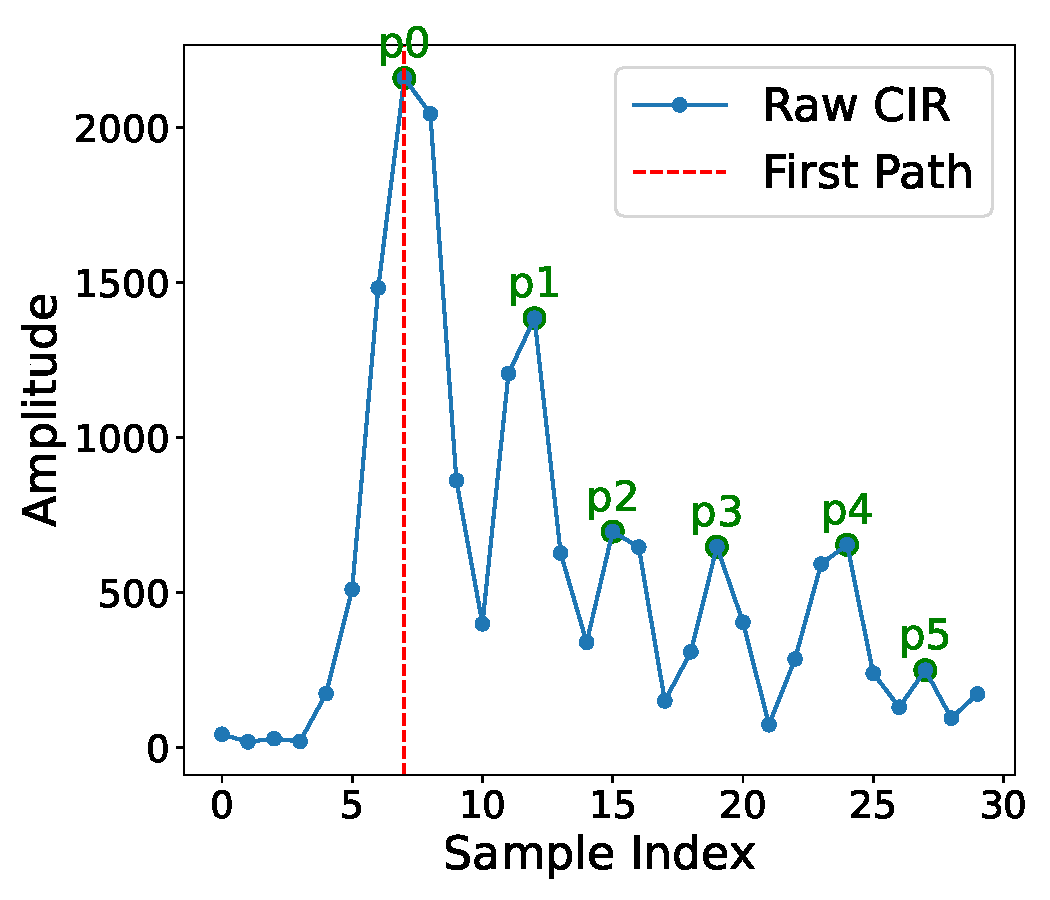
\includegraphics[width=0.95\linewidth]{figures/cir_peaks.pdf}
%   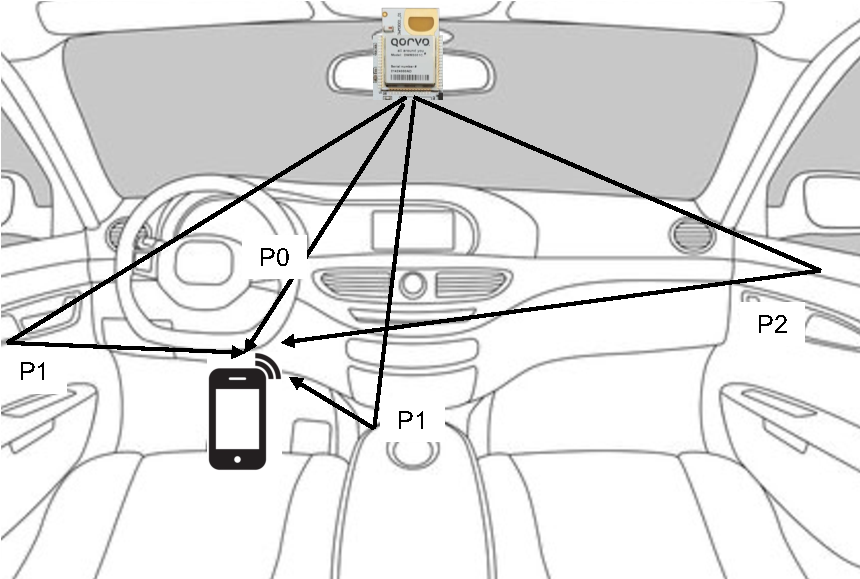
\includegraphics[width=0.95\linewidth]{figures/cir_reflections.pdf}
%     \caption{Peaks show signal reflections from the vehicle interior}
%   \label{fig:cir_reflections}
% \end{figure}

\begin{figure}[t]
  \centering
  \begin{subfigure}[t]{0.4\linewidth}
    \centering
    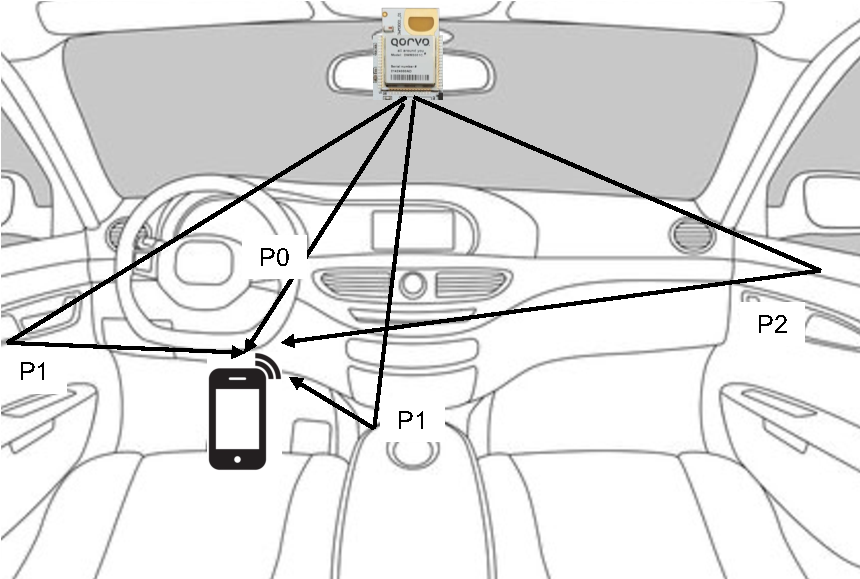
\includegraphics[height=3.3cm]{figures/cir_reflections.pdf}
    \label{fig:cir_reflections_sub}
  \end{subfigure}
  \hfill
  \begin{subfigure}[t]{0.44\linewidth}
    \centering
    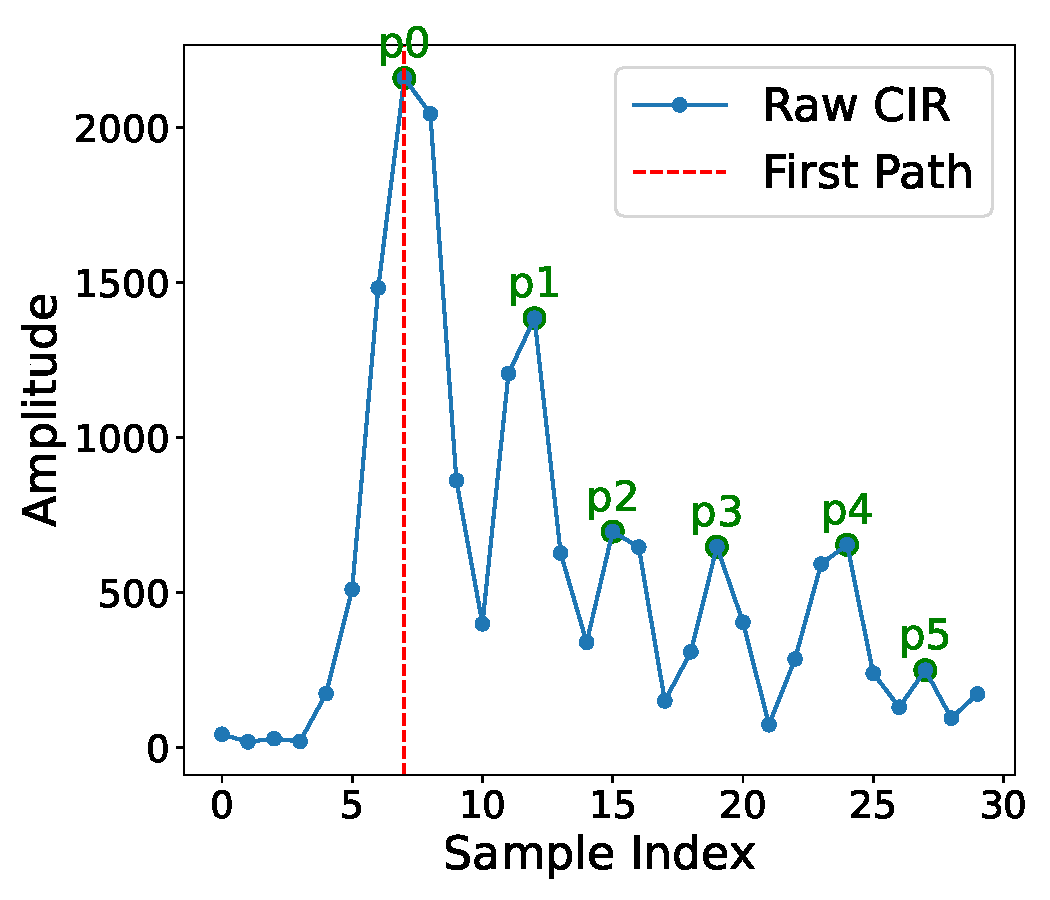
\includegraphics[height=3.3cm]{figures/cir_peaks.pdf}
    \label{fig:cir_peaks}
  \end{subfigure}
  \vp\caption{CIR peaks represent signal reflections from vehicle interior.}
  \label{fig:cir_reflections}
  \vp
\end{figure}




\subsection{Challenges of In-Cabin Phone Localization}
\label{sec:background::challenges}

\name~ aims to reuse the existing in-vehicle UWB infrastructure without 
requiring additional hardware, but this design goal introduces several 
technical challenges as follows.

\textit{Challenge (1): Spatial ambiguity due to number and placement of the
UWB anchor.}
%
% Number of the UWB anchor
Most existing vehicles are equipped with only a single in-cabin UWB anchor 
\cite{Ultra-WidebandCCC}, which is sufficient for identifying whether the 
smartphone/key is in cabin, but limits spatial diversity for fine-grained 
CIR interpretation.
%
When the anchor is centrally located (e.g., at the rearview mirror in 
Fig.~\ref{fig:cir_reflections}), symmetry in the vehicle layout 
exacerbates ambiguity.
%
Fig.~\ref{fig:two_similar_CIRs} compares two CIRs measured from the driver 
and the front passenger seats.
%
Despite vehicles' structural differences (e.g., presence of the steering wheel 
on the driver's side), the CIRs exhibit nearly identical peak features.
%
This is due to the limited time resolution of the commercial UWB transceivers, 
which typically sample CIRs at 1 ns intervals, equivalent to a spatial 
resolution of approximately 30 cm~\cite{Dw3000,UMusic}.
%
Within a 2--3 ns window (60-90 cm), reflections from multiple nearby surfaces 
(e.g., steering wheel, dashboard, and driver side door) merge into a single 
peak in CIR. 
%
Consequently, left and right seating regions may produce indistinguishable
CIR profiles.

\textit{\name~needs to resolve such ambiguity using only a single UWB anchor 
without deploying additional in-cabin UWB anchors.}

\begin{figure}
     \centering
     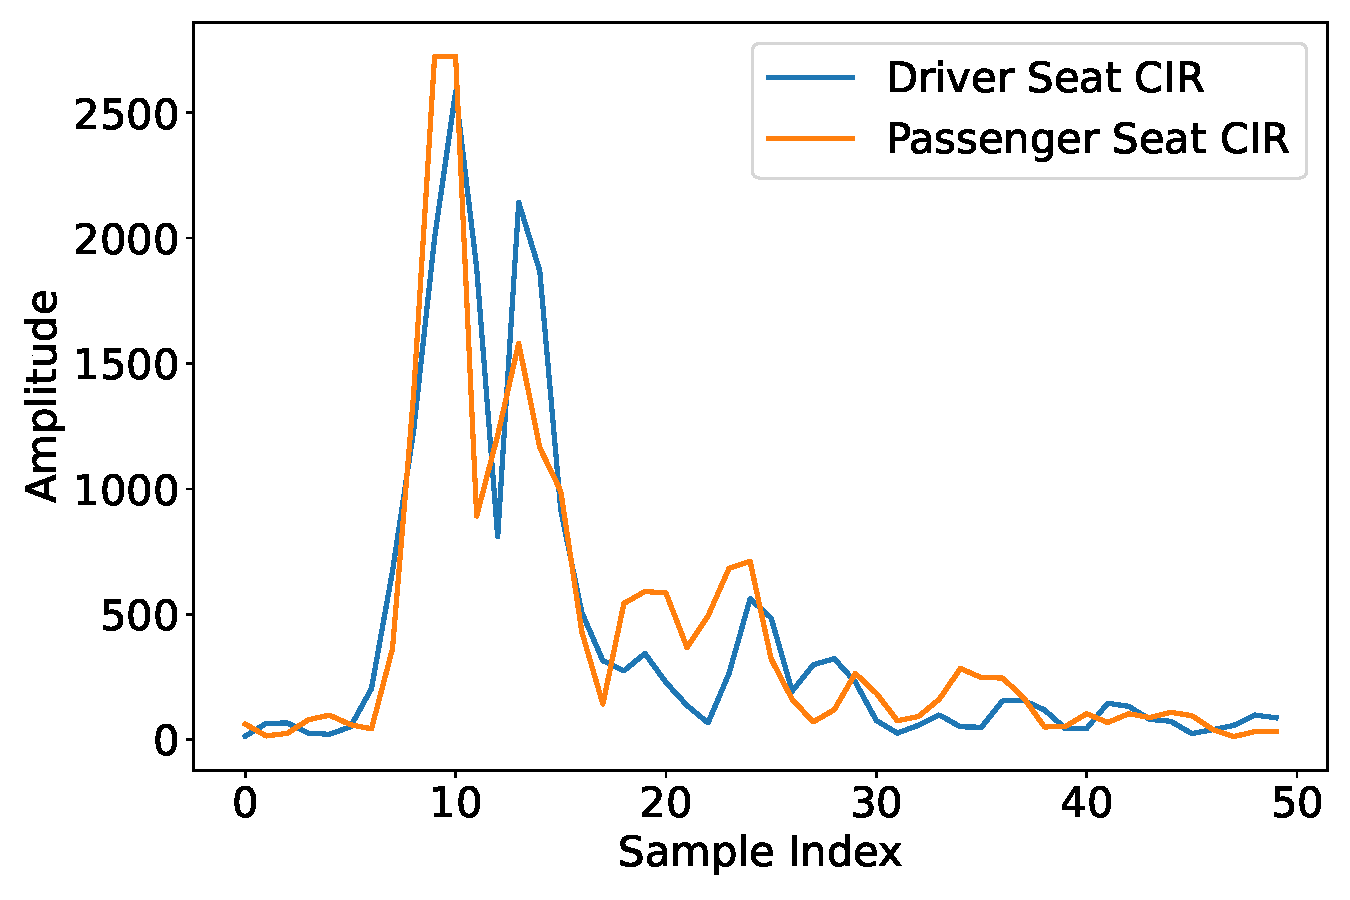
\includegraphics[width=0.7\linewidth]{figures/two_similar_CIRs.pdf}
     \vp\caption{Two CIRs from driver and passenger seat.}
     \label{fig:two_similar_CIRs}
    \vp
 \end{figure}
 
\textit{Challenge (2): Interference caused by human body movement.}
%
In real-world driving scenarios, both drivers and passengers introduce
motion artifacts that significantly impact CIR stability.
%
Drivers frequently move their arms while steering, while passengers often 
interact with their smartphones.
%
In addition, both occupants exhibit large body movements during vehicle
maneuvers such as turns or sudden stops.
%
Furthermore, occupants commonly adjust their seat positions for comfort, resulting 
in changes in in-cabin structure, human posture and relative device position.

These actions cause noticeable perturbations in CIR measurements, 
especially in weaker multipath components.
Fig.~\ref{fig:peak_disappear} illustrates an example of this phenomenon: the 
third peak in the first CIR disappears in the second frame and then reappears 
in the third frame. Such transient changes in peak presence highlight the need 
for robust tracking and smoothing strategies to handle frame-to-frame signal 
variability caused by human motion.

\begin{figure}
    \centering
    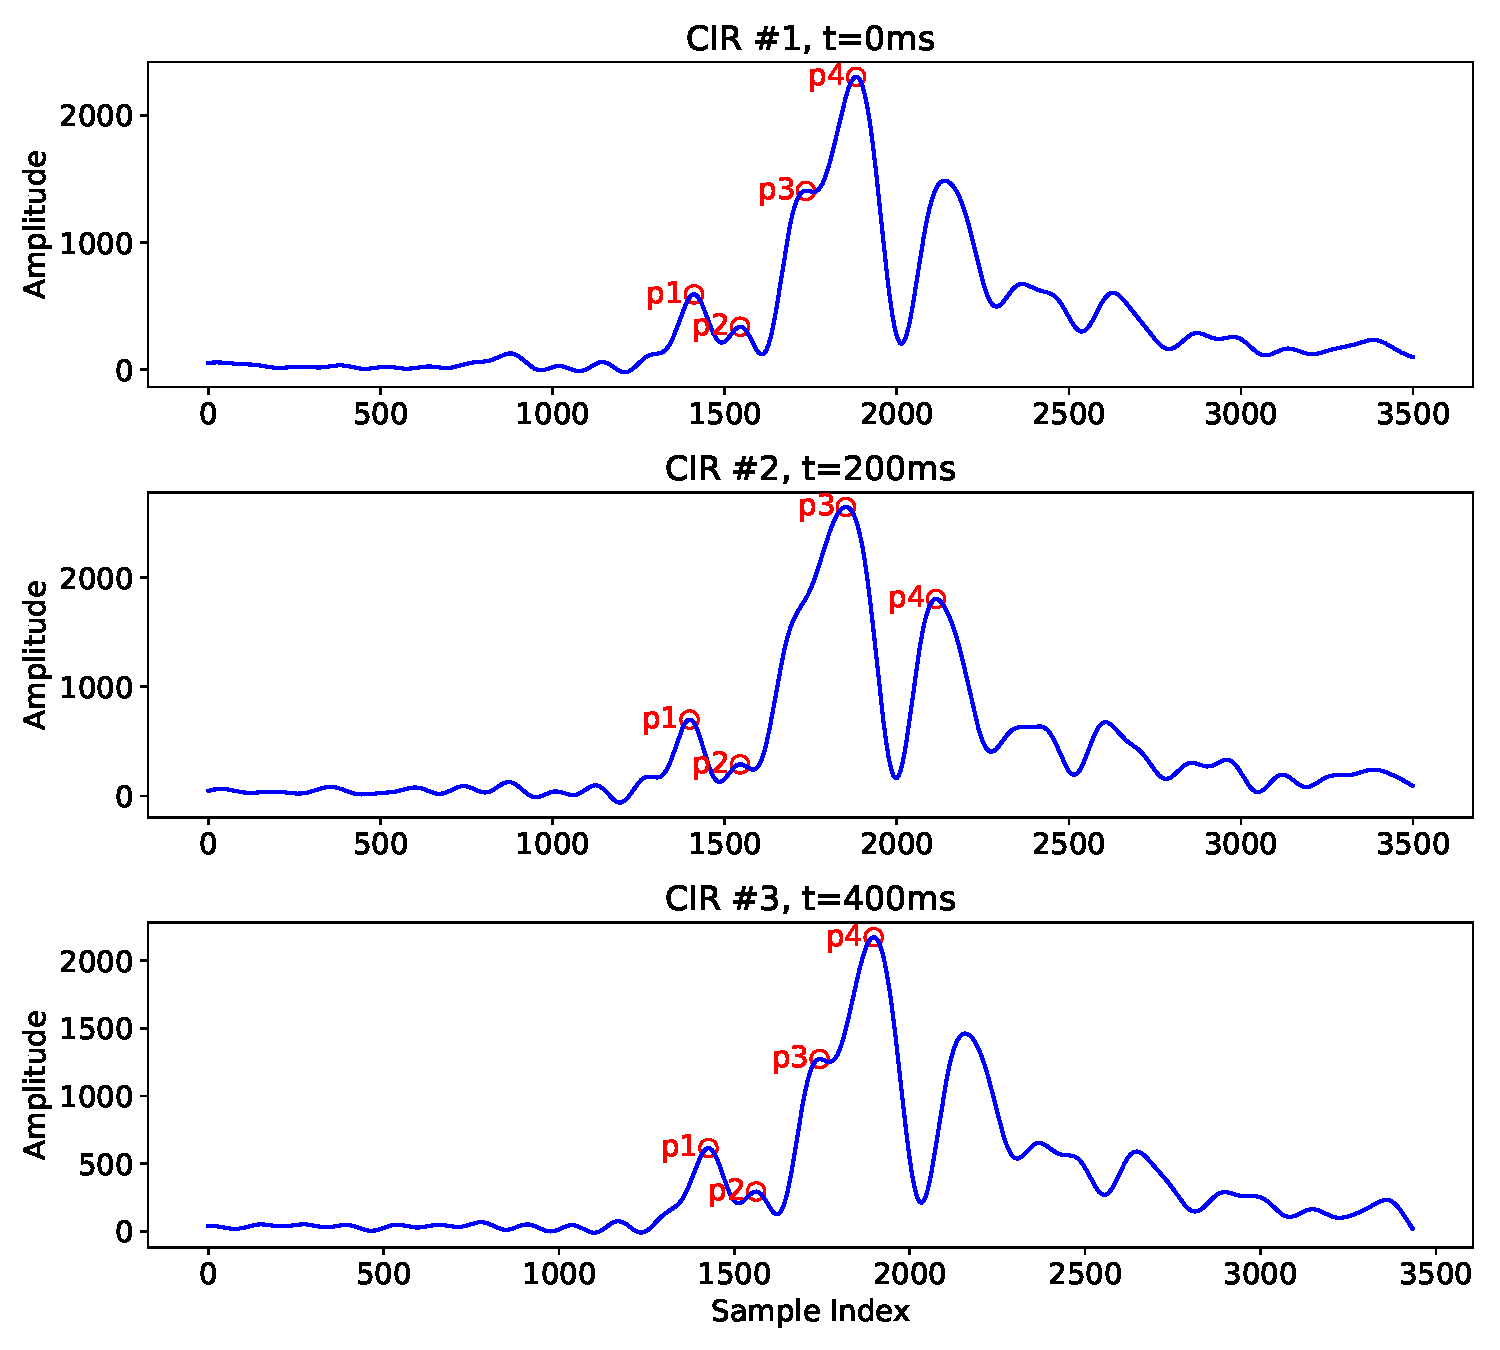
\includegraphics[width=0.9\linewidth]{figures/peak_disappear_timestamped.pdf}
    \vp\caption{\edited{Three consecutive CIRs (200 ms apart) showing the temporary vanishing and reappearance of the third peak.}}
    \label{fig:peak_disappear}
    \vp
\end{figure}


\textit{\name~needs to generalize across a wide range of occupant motions and 
in-cabin layout variations.}

% Location of the UWB anchor
\textit{Challenge (3): Smartphone battery life.}
%
In \name, smartphone functions as both the UWB signal receiver and the
processing unit for localization inference.
%
However, continuous UWB reception and \name~ processing can lead to 
significant battery drain, making the system impractical.
%
The UWB module we use consumes about 160 mW during packet reception 
\cite{polonelli2022performance,Dw3000datasheet}, while Bluetooth consumes 
50--70 mW during active transmission \cite{TI_CC2564MODN}.
In practice, smartphones minimize UWB active time. For example, 
the UWB-based car Digital Key system use Bluetooth LE for presence 
detection and wake the UWB radio only for a quick distance verification \cite{apple_uwb_car_keys_2021}.


\textit{\name\ must, therefore, incorporate an intelligent triggering
mechanism for phone localization only when necessary.}

% \section{Background and Challenges}
% \label{sec:background}


% \subsection{UWB Background}
% Ultra‐Wideband (UWB) is a radio‐frequency (RF) technology designed to support precise distance measurements via time‐of‐flight (ToF) \cite{coppens2022overview}. Automotive manufacturers increasingly integrate UWB into vehicle keyless entry systems \cite{Bmw_2022,tesla_model3_manual_2025,hyundai_digital_key_2025}, primarily serving two functions: localizing the approaching owner for convenience and welcoming features \cite{ghabra2020apparatus,apple_uwb_car_keys_2021}, and securely verifying the owner's proximity within the vehicle to prevent relay attacks a vulnerability associated with older wireless key fobs \cite{fira_digital_key_2024,francillon2011relay}. Although specific UWB configurations by car manufacturers remain proprietary, typically these keyless systems deploy multiple external anchors to localize approaching users and one internal anchor dedicated to secure ranging with the owner's smartphone \cite{Ultra-WidebandCCC, golsch2019passive}.

% Existing state-of-the-art UWB localization solutions rely either on multiple anchors using Time-Difference-of-Arrival (TDoA) methods \cite{chantaweesomboon2016performance,kempke2016surepoint,tiemann2016atlas} or single anchors equipped with multiple antennas leveraging Angle-of-Arrival (AoA) \cite{ge2021single,cao2020accurate,arun2023xrloc,zhao2021uloc}. However, current UWB keyless entry systems hardware are not designed for localization of smartphones \emph{inside} the vehicles. The external anchors are optimized for outdoor localization, and their internal coverage depends heavily on manufacturers' specific configurations. Additionally, the single internal anchor is typically limited to basic ranging functions, without support for AoA measurements. Then, how can we leverage this single, basic transceiver to achieve seat-level localization inside the vehicle? One approach is multipath profiling.

% \subsection{Use of CIR for Localization}

% Upon receiving a packet, a UWB transceiver records CIR, a time-domain snapshot 
% capturing the multipath propagation of the UWB signal within a short window (1,016 ns) 
% %CCCC Where did this number come from?
% surrounding packet reception \cite{Dw3000}. The CIR records the received signal 
% at 1 ns intervals. The first peak indicates the arrival of a direct signal from 
% %CCCC Why 1ns interval?
% the transmitter. The secondary peaks correspond to signal reflections arriving at 
% the transceiver \cite{schmidt2024salos,schmidt2019effective,grosswindhager2018salma}. 
% The indices of secondary peaks indicates the delay of reflected path propagation. 
% The amplitudes of secondary peaks indicate signal attenuation along those paths.
% As shown in Fig.~\ref{fig:cir_reflections}, the first peak indicates the direct
% path signal. The reflections from closely spaced front surfaces (e.g., central 
% console and front doors) merge into a single peak (p1), while later peaks (p2, p3, p4) 
% represent reflections from more distant surfaces like driver's side door, ground, 
% rear area or trunk. In this way, CIR encodes information about signal propagation 
% paths from the transceiver to the smartphone, which can be used to profile each
% different smartphone location inside the car.




% Prior research has demonstrated feasibility for single-anchor 
% localization with CIR. For example, single-anchor localization systems proposed 
% in \cite{grosswindhager2018salma,schmidt2024salos} collect both ranging results and  
% CIR data from a single UWB anchor. These systems identify candidate locations on 
% a circle with a radius equal to the measured ranging distance, and then model 
% theoretical multipath propagation at each candidate location. 
% The location is estimated by comparing these theoretical CIR profiles with the
% measured CIR and then selecting the candidate point with the closest CIR match.
% Using a single basic UWB transceiver as an anchor, \cite{grosswindhager2018salma}
% achieved a 70th percentile accuracy within ±30 cm.

% But vehicle interiors present more complex multipath environments than typical 
% indoor environments due to irregularly shaped, angled reflective surfaces 
% such as dashboards, seats, and consoles. This complexity results in dense, 
% overlapping multipath signals that are difficult to model explicitly for every 
% possible location. Given that the vehicle cabin is a constrained environment with
% only a limited number of possible smartphone locations, and that our goal is 
% to prevent driver phone use, we propose to train a ML 
% model to perform binary classification between driver and passenger seats 
% %CCCC Sat why binary classification (explained)
% rather than pure localization (calculating coordinates of phone). Then, how can we profile signal propagation characteristics that are unique to the driver's seat? 

% \subsection{Challenges in CIR-based In-vehicle Localization}

% We face several unique challenges in achieving CIR-based seat-level classification inside a vehicle. 
 
% Seat-level CIR profiling aims to leverage the physical differences in signal 
% propagation paths between the UWB anchor and each seat location, so that a ML 
% model can distinguish driver and passenger phone locations based on CIR features. 
% At a first glance, the front row of a vehicle appears geometrically asymmetric,
% e.g., the steering wheel, dashboard contours, and center console are primarily 
% located on the driver's side. Based on this, we initially hypothesized that such 
% asymmetries would produce distinct CIR profiles, particularly in the indices 
% of early CIR peaks.
 
% In practice, however, this assumption does not hold when the UWB anchor is placed 
% at a central location, such as near the rearview mirror, which is common 
% in production vehicles \cite{fcc_audi_uwbtrx22_2021,fcc_bmw_fbd5_2021}. 
% The CIR is sampled every 1 ns, corresponding to roughly 30 cm in signal path
% difference. Given that the steering wheel, dashboards and driver side door are 
% separated by approximately 50–-80 cm, multipath signal components reflecting off 
% these surfaces arrive within 2--3 ns of each other and merge as a single CIR peak. 
% Thus, two regions on the left and right side of the car may produce CIRs with 
% similar peak indices, as shown in Fig.~\ref{fig:two_similar_CIRs}. 
 
 
 

% To resolve this ambiguity, we develop a seat-level smartphone localization system 
% that adapts to different anchor locations by intentionally generating 
% asymmetry into the signal-propagation environment.
% \begin{itemize}
%   \item When anchor placement is flexible (e.g., in aftermarket solutions or future 
%     vehicle designs), we identify effective anchor locations and combine them with 
%     a robust CIR processing pipeline to enhance signal path distinctiveness 
%     between driver and passenger seats.
%   \item When anchor placement is inflexible/fixed (e.g., production vehicles 
%     with a built-in UWB transceiver), we add a small metal 
%     shield that attenuates signals toward one side of the vehicle and reflects 
%     them toward the other. 
%     This passive modification creates distinguishable signal propagation profiles 
%     between driver and passenger seats, enabling accurate classification even 
%     when CIR resolution limits prevent the separation of peaks.
% \end{itemize}

 % CIR is also susceptible to noises caused by changes in the multipath environment inside the vehicle. Reflected signal paths can be blocked by human body or vehicle parts such as steering wheel, leading to temporary disappearance and shifting of CIR peaks even when the phone stays still. We need to mitigate the impact of temporarily disappeared peaks and detect noisy CIRs. 

% \subsection{Other Challenges: Toward a Usable and Efficient System}
% Besides classification accuracy, a practical smartphone localization system must 
% also be efficient and usable. Continuous UWB ranging drains phone battery and may 
% be unnecessary if the phone remains stationary throughout the trip.
% The system must, therefore, automatically trigger phone localization only when 
% necessary --— specifically, when the phone moves across seats. 

% \textbf{Summary.} Overcoming the above technical challenges has led to our 
% development of \name: a smartphone-based seat-level localization system that uses 
% a {\em single} in-vehicle UWB anchor. It integrates efficient motion-triggered 
% activation, robust CIR feature extraction and ambiguity mitigation/resolution
% through anchor placement and/or a mounted shield on the UWB anchor.

% For vehicles equipped with an internal UWB transceiver, we provide a guideline 
% for assessing the driver--passenger seat ambiguity. If anchor placement is prone
% to this ambiguity, adding a simple metal shield will enable seat-level classification. 

\section{System Design}

\begin{figure*}[htbp]
    \centering
    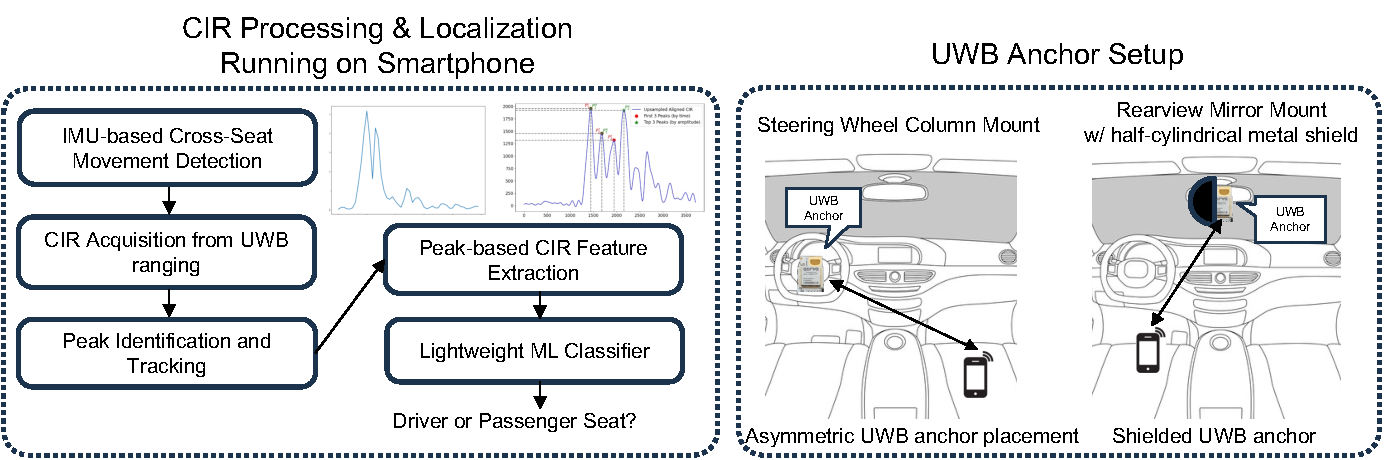
\includegraphics[width=0.9\textwidth]{figures/overview_wider.pdf}
    \vspace{-10pt}
    \caption{System overview.}
    \label{fig:overview}
    \vp
\end{figure*}

This section describes the system design of \name.
%
Fig.~ \ref{fig:overview} shows the e2e workflow of \name, 
which is implemented as a smartphone app.
%
First, the smartphone uses its onboard IMU sensors to intelligently decide when 
to initiate self-localization (Challenge (3), Section~\ref{sec:system::trigger}).
%
Then, it processes the received UWB CIR to perform seat-level localization, 
ensuring robustness against motion artifacts (Challenge (2),  
Section~\ref{sec:system::localization}).
%
Finally, we propose a method to create signal asymmetry while minimizing 
modifications to the existing UWB anchor infrastructure, thereby resolving 
CIR ambiguity (Challenge (1), Section~\ref{sec:system::asymmetry}).

\subsection{Detection of Seat-Level 
Phone Location Changes} \label{sec:system::trigger}
%
\name~aims to maintain accurate seat-level localization of the smartphone 
while minimizing energy consumption.
%
Once the phone's initial location is established, continuous localization is 
unnecessary. \name\ leverages low-power IMU sensors to opportunistically trigger 
UWB-based localization only when it detects the phone has moved across seats.
%
Unlike prior work that detects general phone movement to trigger localization 
\cite{kim2010sensloc, zhuang2010improving}, \name\ targets fine-grained 
detection of cross-seat movements within a vehicle cabin.
%
Our design goal is to avoid false negatives, which would result in undetected
seat changes and ultimately localization and tracking failures, while
minimizing false positives that incur unnecessary localizations.

To meet this requirement, \name\ employs a lightweight IMU-based detection model 
that differentiates cross-seat phone movements from common motion sources 
such as normal vehicular dynamics and in-hand phone manipulations.
%
To guide the model design, we first conducted real-world experiments to 
characterize IMU signatures under three scenarios: 1) cross-seat phone movement; 
2) phone manipulation while held in hand, and 3) in-hand phone movement 
during vehicle acceleration.
%

%
Each scenario was performed 40 times inside a moving vehicle along urban and 
suburban roads. For cross-seat movement, we tested transitions both during 
vehicle stops and while the car was in motion, including cases where the user 
reached across the cabin, passed the phone to a neighboring seat, or moved the 
phone to and from cup-holder area. For in-hand manipulation, we performed 
typical phone usage actions such as unlocking, scrolling, or adjusting the phone's 
orientation. For the vehicle-induced condition, users held the phone loosely in a 
natural posture during acceleration, braking, or turns without actively moving it.

Our design is based on three core observations.

(1) Cross-seat phone relocations typically occur over short durations.
%
We empirically chose a window size of 1.2 seconds with a step size of 0.2 second 
for IMU processing, with data sampled at 50Hz.
%
This is sufficient to capture the full duration of most cross-seat movements,
while minimizing the inclusion of unrelated motion.

(2) Motion generated by the vehicle itself (e.g., acceleration or 
cornering) rarely produces strong gyroscope activity when the phone is stationary.
%
In contrast, user-initiated movements (e.g., picking up or moving the phone) 
result in significant rotational changes.
%
\name\ first filters out vehicle-only motion by applying a gyroscope magnitude 
threshold to detect phone pick-up events.

(3) Cross-seat movements tend to be brief, abrupt, and generate high 
accelerometer variability, distinguishing them from more subtle 
in-hand manipulations.
%
\name\ uses the standard deviation of accelerometer magnitude within the detection 
window to further discriminate between in-seat handling and actual relocation.
%
A conservative threshold is chosen based on the empirical experiments 
(see Fig.~~\ref{fig:accel_thresholds}) to suppress false positives while 
ensuring reliable detection of seat-level transitions.

\begin{figure}[t]
\centering
\includegraphics[width=0.85\linewidth]{figures/accel_thresholds.png}
\vp\caption{Net displacement vs.~standard deviation of acceleration 
in 120 movement events.}
\label{fig:accel_thresholds}
\vp
\end{figure}

\subsection{Motion-Resilient %CIR-Based 
Phone Localization} \label{sec:system::localization}
%
Once triggered, \name\ processes the raw CIR data to extract multipath 
features for seat-level smartphone localization.

\textbf{CIR Preprocessing}:
%
We begin by identifying the index of the first significant CIR peak 
($\text{fp}_{\text{index}}$), typically corresponding to the LoS path 
from the UWB anchor to the smartphone.
%
Given the constrained in-cabin environment, we narrow the analysis window to 
a segment around the LoS path, specifically $[\text{fp}_{\text{index}} - 10, 
\text{fp}_{\text{index}} + 40]$, which corresponds to propagation distances 
within approximately $12$m.
%
To improve spatial resolution, we upsample the CIR waveform by a factor of 
$64$ using interpolation techniques, enabling finer peak discrimination 
\cite{kalyanaraman2020caraokey,cao2024utrack3d}.

\textbf{CIR Feature Extraction}:
As discussed in Section \ref{sec:background}, CIR peaks characterize 
reflections from in-cabin structures.
%
The relative positions (index differences) and amplitudes of these peaks 
encode the propagation delay and signal attenuation of multipath components.

We use a set of features proposed in \cite {kalyanaraman2020caraokey}.
\name\ extracts the top $n=4$ CIR peaks based on amplitude and sorts them by index. 
%
For each non-primary peak, it computes the index offset and amplitude ratio 
relative to the first peak. 
%
These features reflect the spatial arrangement and reflectivity of nearby surfaces.
%
Fig.~\ref{fig:cir_features} shows the features extracted from the top four peaks of a CIR. 

\begin{figure}
    \centering
    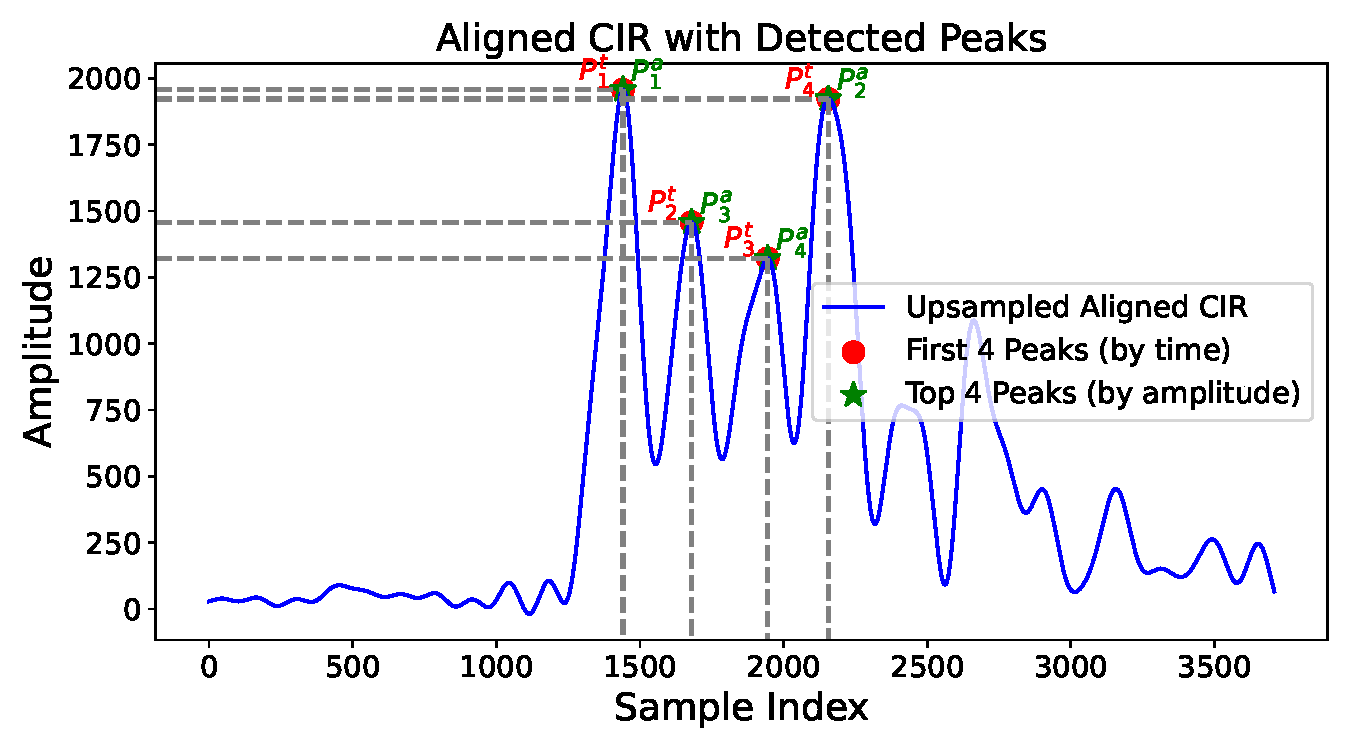
\includegraphics[width=0.9\linewidth]{figures/cir_features_wider.pdf}
    \vp\caption{Features based on top 4 peaks.}
    \label{fig:cir_features}
    \vspace{-0.2in}
\end{figure}
%
% Peaks beyond the fourth are often due to reflections from external surfaces such as the trunk or ground and to maintain in-cabin relevance. 
Peaks beyond the fourth are typically the result of long-path reflections, often 
from the vehicle floor, trunk, or exterior structures. They are excluded as 
these late components exhibit lower amplitude and higher variability.
%
In addition to CIR-based features, we also include the ranging distance between the anchor and smartphone, which provides a coarse location prior.
%
The complete set of features used in classification is summarized in Table~\ref{tab:CIR_features}.

% \begin{table}[]
% \caption{Features extracted from CIR.}
% \label{tab:CIR_features}
% \vp\small
% \setlength\tabcolsep{1.8pt}
% \begin{tabular}{|l|}
% \hline
% \textbf{Features description }                                      \\ \hline
% Index separation from first peak (first $n$ peaks by time)                \\ \hline
% Amplitude ratio to first peak (first $n$ peaks by time)                   \\ \hline
% Index separation from highest amplitude peak (top $n$ peaks by amplitude) \\ \hline
% Amplitude ratio to highest amplitude peak (top $n$ peaks by amplitude)    \\ \hline
% Number of detected peaks                                                \\ \hline
% Index of highest amplitude peak                                         \\ \hline
% Amplitude of highest peak                                               \\ \hline
% \end{tabular}
% \end{table}
\begin{table}[]
\caption{Features used for classification.}
\label{tab:CIR_features}
\vp\small
\setlength\tabcolsep{1.8pt}
\begin{tabular}{|l|}
\hline
\textbf{Features description}                                      \\ \hline
Ranging distance between anchor and smartphone                    \\ \hline
Index separation from first peak (first $n$ peaks by time)        \\ \hline
Amplitude ratio to first peak (first $n$ peaks by time)           \\ \hline
Index separation from highest amplitude peak (top $n$ by amplitude) \\ \hline
Amplitude ratio to highest amplitude peak (top $n$ by amplitude)  \\ \hline
Number of detected peaks                                          \\ \hline
Index of highest amplitude peak                                   \\ \hline
Amplitude of highest peak                                         \\ \hline
\end{tabular}
\vspace{-15pt}
\end{table}


\textbf{Robust Inter-frame CIR Peak Tracking}:
%
 While peak indices are key features for location classification, they are susceptible to disruption from occupant motion or environmental changes.
%

%
These disruptions may cause peaks to temporarily vanish, reappear, or shift 
between consecutive CIRs, even when the phone remains stationary.
%
\edited{Fig.~\ref{fig:peak_disappear} shows an example of this phenomenon: 
three CIRs are captured 200 ms apart while the phone is held at the same 
location, but the third peak in the first CIR disappears in the second
frame and reappears in the third frame.}
%
This variability arises from two common effects: (i) temporary occlusion of 
reflection paths by body parts (e.g., a driver’s arm), and (ii) resolution 
limitations when multiple reflection paths arrive within a narrow time 
window (e.g., $<1$ns), leading to peak merging or separation across 
frames \cite{cao2024utrack3d}.
%
Because \name's classification features rely directly on peak stability, 
such fluctuations degrade the consistency of extracted feature vectors.
%
To mitigate this, \name\ implements \textbf{inter-frame peak tracking},
which stabilizes peak detection by preserving temporarily missing peaks 
and smoothing out transient variations. 
\edited{This method leverages the strong resemblance in peak positions 
across consecutive CIRs when the phone's location and the in-cabin 
propagation environment are quasi-static.}

For each new CIR measurement, local maxima are identified beyond the first 
peak index using an amplitude threshold.
%
Each detected peak is then compared against a record of previously tracked peaks. 
%
To avoid incorrect matches with adjacent peaks, if a new peak lies within a 
tolerance window of an existing peak, it is treated as the same and its position 
is updated. 
%
Since two peaks are separated by at least 2 indices (128 after 
upsampling by a factor of 64), we empirically set tolerance window to 
100 indices to accommodate minor peak jitter while ensuring that the peak 
is not matched with an adjacent peak. 
%
\edited{This window is wide enough to accommodate minor peak jitter from small motions, yet narrow enough to avoid incorrect matches with adjacent peaks.}
%
If no match is found, a new peak entry 
is added. Unmatched old peaks are retained against brief disappearance.
Fig.~\ref{fig:peaktracking_track} shows three consecutive CIR measurements, \edited{where the algorithm successfully preserves the third peak despite its temporary disappearance in CIR~\#2.}
% \edited{Note how the algorithm preserves the third peak through 
% a temporary disappearance in CIR \#2.}
% The third peak in CIR 2 is retained.

\begin{figure}
    \centering
    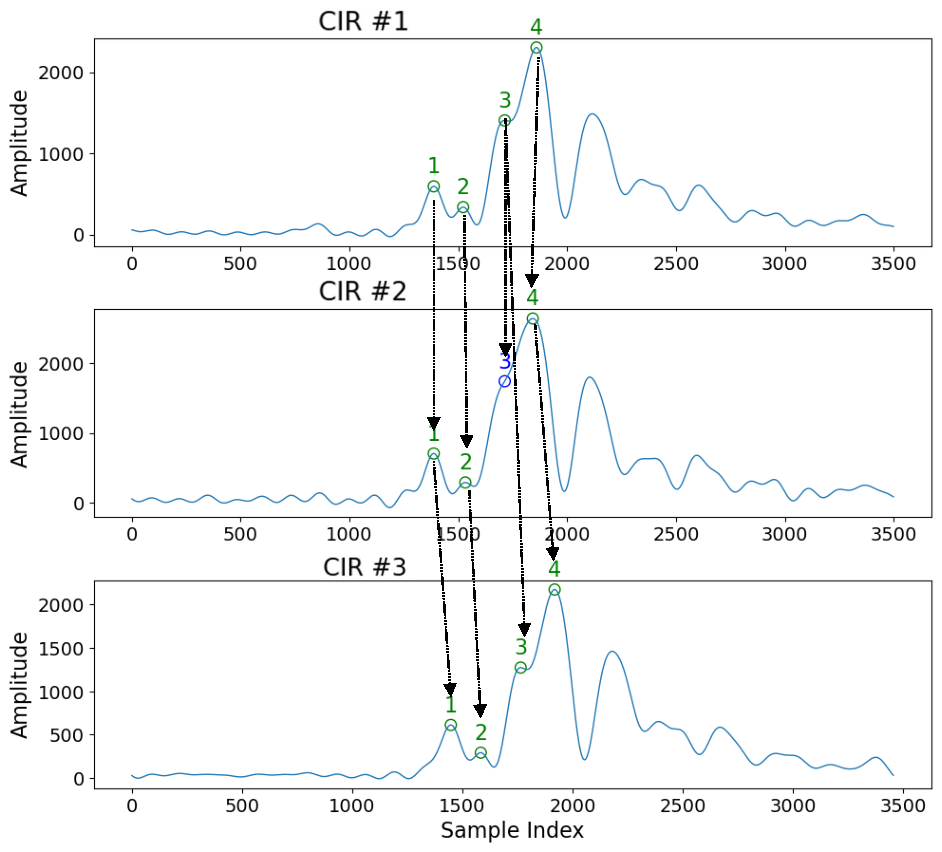
\includegraphics[width=0.9\linewidth]{figures/peaktracking.pdf}
    \vp\caption{Three consecutive CIRs with peaks tracked.}
    \label{fig:peaktracking_track}
    \vp
\end{figure}

% This tracking method significantly reduces the variance of CIR-based features over time.
%
We analyze the stability of our extracted peak indices with and without 
inter-frame peak tracking by using consecutive five CIR measurements from our  testing dataset (details in Section~\ref{sec:evaluation:methodology}).
%
Fig.~\ref{fig:feature_variance} shows results of three inter-peak time difference 
features: $\Delta t_1$, $\Delta t_2$, and $\Delta t_3$, representing the index 
separations between the first peak and the second, third, and fourth peaks,
respectively.
%
The standard deviation of $\Delta t_3$ drops from $127.1$ ($\approx$0.6 m) to 
$82.7$ ($\approx$0.4m) indices after tracking is applied, with similar improvements 
observed for $\Delta t_1$ and $\Delta t_2$. 
%
This enhanced stability improves classification robustness under motion 
artifacts (see detailed experiments in Section~\ref{sec:evaluation:accuracy:occupant}), especially when a 
passenger is present.

However, when the smartphone changes position, CIR peak indices 
need to reflect this change.
%
If old peaks are blindly preserved, they may distort the localization output.
%
\name\ needs to distinguish between temporary peak disappearance and peak 
shifting due to change in the smartphone’s location.
%
Our empirical observations suggest that a genuine phone movement typically 
causes multiple peaks to shift beyond the matching tolerance, reflecting a
true change in the spatial configuration of reflective paths, as shown 
in Fig.~\ref{fig:peaktracking_unstable}, peak 2 and peak 4 of the second CIR 
has shifted beyond the matching tolerance.
%
\begin{figure}[t]
    \centering
    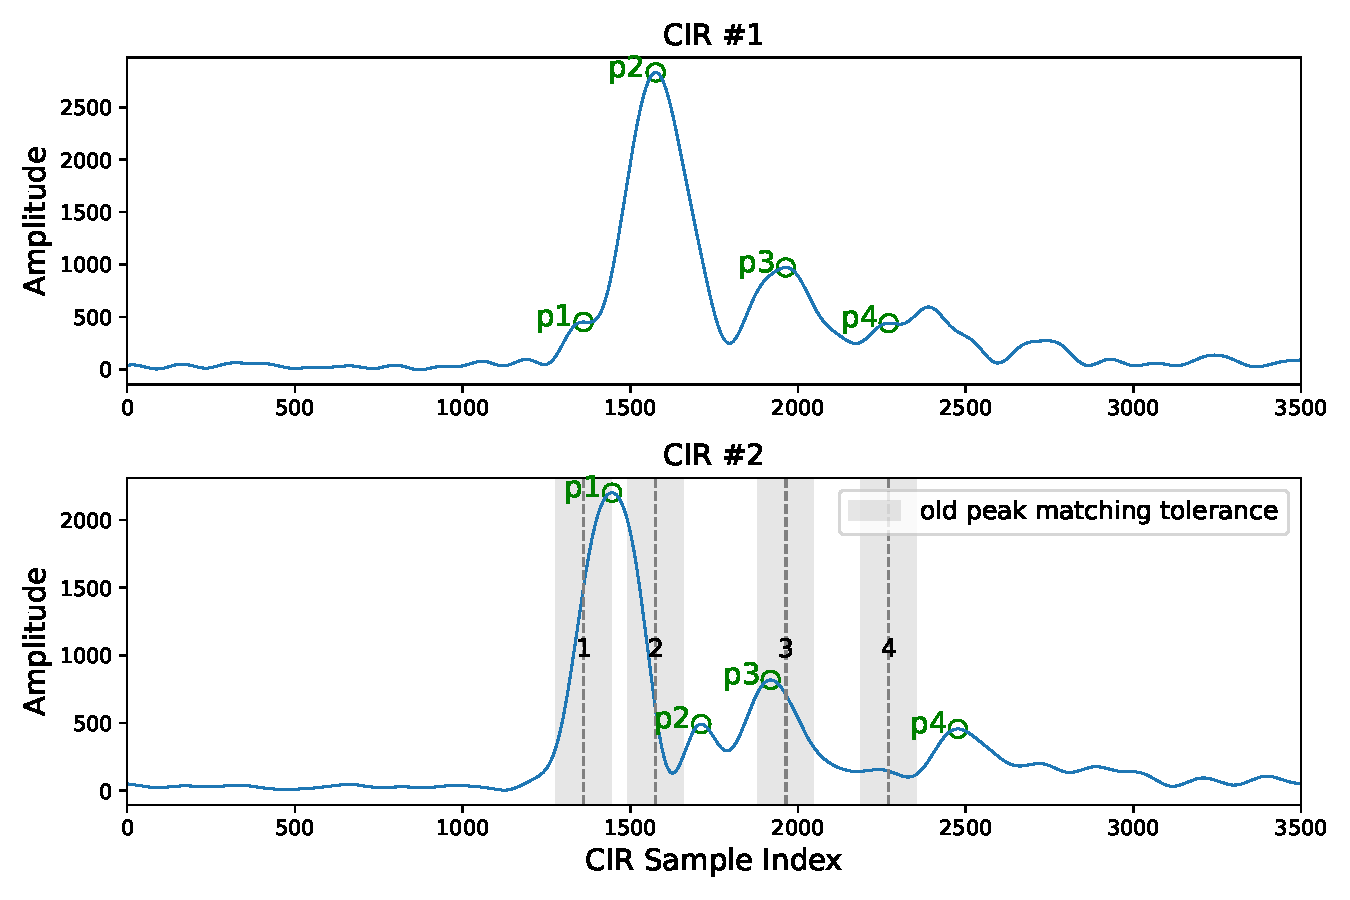
\includegraphics[width=0.9\linewidth]{figures/peaktracking_unstable.pdf}
    \vp\caption{Two peaks become unstable in CIR 2.}
    \label{fig:peaktracking_unstable}
    \vp
\end{figure}

In contrast, during stationary conditions, most peaks remain stable across frames.
%
We verify this by collecting $200$ CIRs, with $100$ the phone is stationary 
and another $100$ during deliberate phone movement, respectively.
%
Fig.~\ref{fig:unmatched_histogram} shows the distribution of unstable peaks 
in these two scenarios, where the unstable peaks mean that the CIR peak 
indices exceed the matching tolerance. We record the number of unstable peaks in each frame. This measurement helps 
\name~distinguish true location changes from transient noise, ensuring both 
responsiveness and resilience in the presence of motion.
%
When more than one of the first 4 peaks becomes unstable, the CIR is 
marked unreliable for localization and will be skipped.
%

\begin{figure}[t]
  \centering
  % \begin{subfigure}[t]{0.48\linewidth}
  \begin{minipage}{0.48\linewidth}
    \centering
    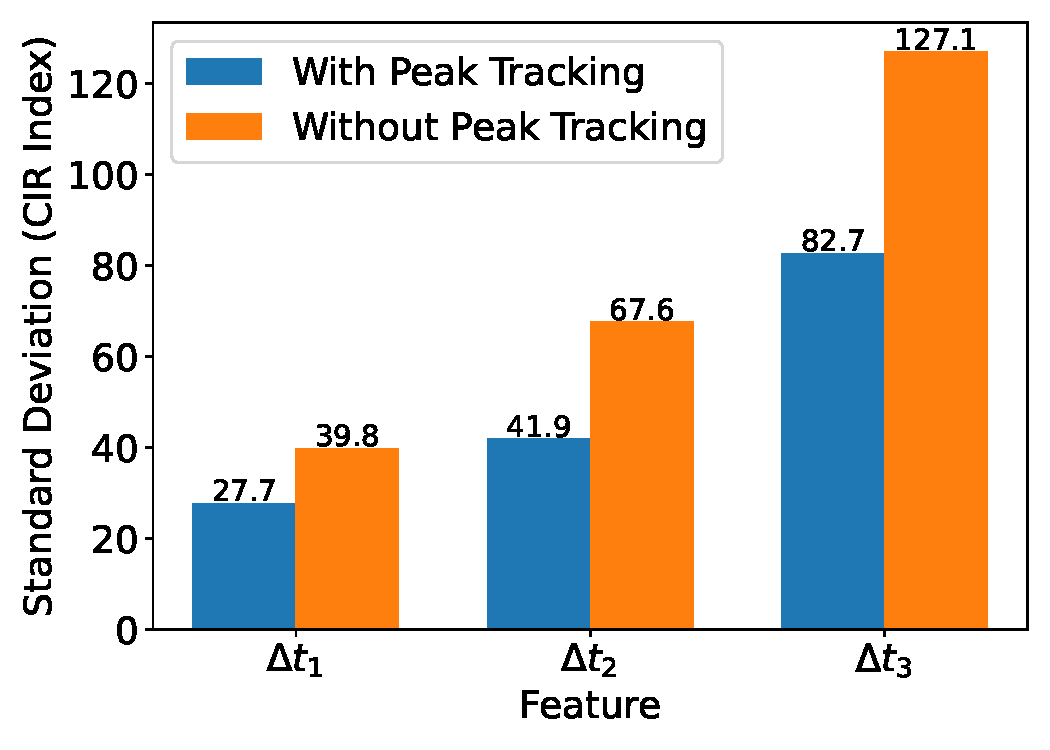
\includegraphics[width=\linewidth]{figures/cir_variance.pdf}
    \vp\vp\caption{Feature SD over 5 consecutive CIRs.}
    \label{fig:feature_variance}
  \end{minipage}
  % \end{subfigure}
  \hfill
  % \begin{subfigure}[t]{0.48\linewidth}
  \begin{minipage}{0.48\linewidth}
    \centering
    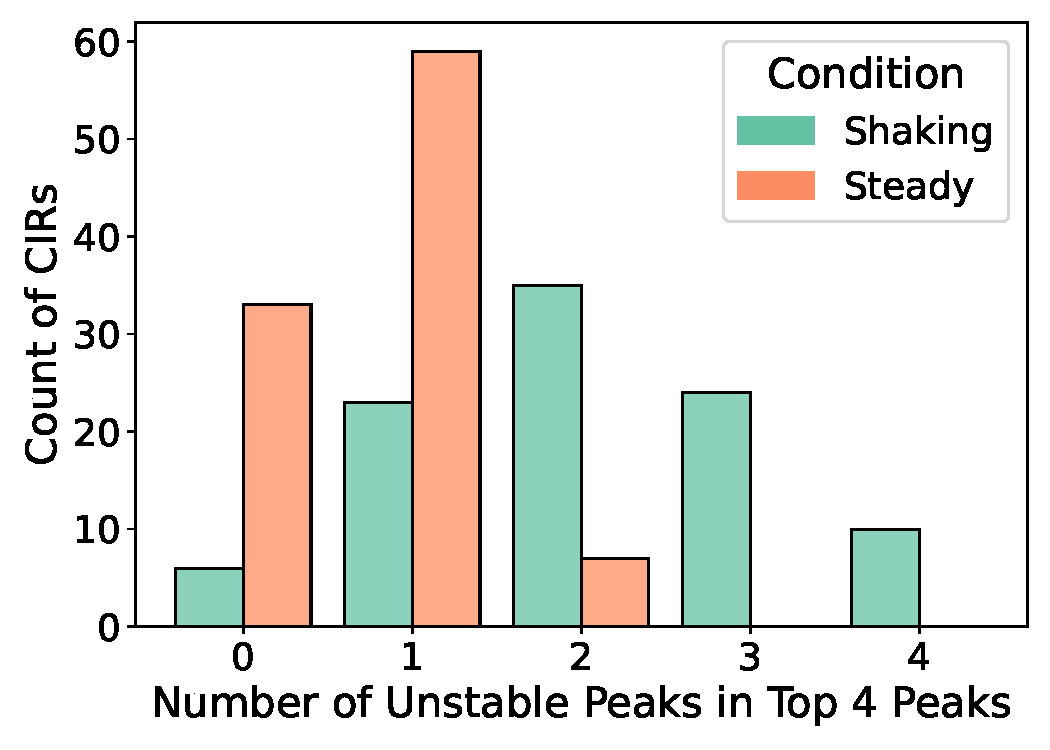
\includegraphics[width=\linewidth]{figures/unmatched_histogram.pdf}
    \vp\vp\caption{Unstable peaks when shaking vs. steady.}
    \label{fig:unmatched_histogram}
  \end{minipage}
  % \end{subfigure}
  % \vp\caption{(a) How peak tracking reduces feature variance and (b) Unstable peaks imply phone movement}
\vspace{-20pt}
\end{figure}

\edited{
We summarize the CIR peak tracking pipeline as follows.
\begin{enumerate}
    \item \textbf{Detect and Compare:} For each new CIR frame, detect all 
    candidate peaks and compare them against a list of previously 
    tracked peaks.
    \item \textbf{Assess Stability:} Count the number of tracked peaks that 
    have shifted beyond a predefined matching tolerance window, indicating 
    a significant change in the multipath profile.
    \item \textbf{Update or Skip:} If there are more than one shifted peaks
    in a frame, the frame is marked as \textbf{unreliable}, and the
    localization is skipped to avoid classifying during motion. 
    Otherwise, the list of tracked peaks is updated with their new 
    positions, and this stable list is used for feature extraction.
\end{enumerate}
}

Overall, through inter-frame peak tracking, we maintain a steady multipath 
profile at one location under environment noises and detecting smartphone’s
actual location change, and only localize the phone when it remains steady, 
reducing misclassifications when smartphone is moving.



\textbf{Multi-Phone Localization}:
The extracted features (Table \ref{tab:CIR_features}) allow us to train a lightweight ML model that can be
run in real time on the phone. 
Since our extracted CIR features are nonlinear, we choose the Random Forest
model (100 estimators) as it handles nonlinear decision boundaries effectively 
through its ensemble of decision trees. The classifier outputs a binary label 
indicating whether the phone is on the driver or passenger side.

%
\name\ can also localize multiple smartphones in a round-robin manner. 
%
While the off-the-shelf anchor can only respond to one phone at a time, 
we implement a wait-and-reconnect protocol in the smartphone app. 
%
If the anchor is currently ranging with another phone, the waiting 
device retries connection after a short delay. 
%
In practice, since localization is triggered infrequently, only when the 
phone moves across seats, the round-robin scheduling does not introduce 
noticeable ranging delays  (Section~\ref{sec:evaluation::End-to-end}).

\subsection{Resolving Ambiguity by Creating Asymmetry for In-cabin UWB Sensing} \label{sec:system::asymmetry}

\begin{figure}[t]
  \centering
  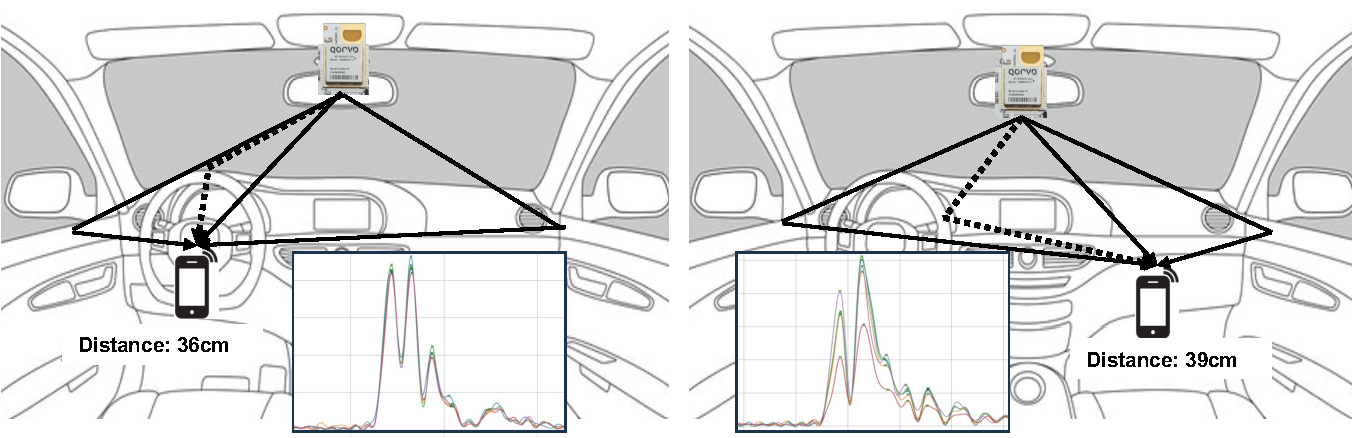
\includegraphics[width=\linewidth]{figures/ambiguity_cir.pdf}
  \vp\caption{Two locations with overlapping CIR and distance.}
  \vspace{-10pt}
  \label{fig:ambiguity_cir}
  \vp
\end{figure}

\name~is designed to repurpose the existing single-anchor UWB 
infrastructure for in-cabin smartphone localization.
%
A core challenge in this setting arises from the inherent spatial symmetry of
the vehicle cabin, particularly between the driver and front passenger seats,
which results in similar UWB propagation characteristics and introduces 
localization ambiguity (see Section~\ref{sec:background::challenges}).
%
To overcome this, we explore two complementary approaches: (1) optimizing the 
anchor location at design time, and (2) applying a directional RF shield in 
retrofit scenarios. We focus on resolving ambiguity between driver and passenger 
seat on the front row, \edited{as back-row locations can be easily distinguished by their significantly longer UWB ranging distances.}
%
Together, these strategies enable robust and low-cost in-cabin smartphone 
localization without modifying the UWB hardware.

\subsubsection{Optimizing UWB Anchor Placement}
%
We first consider a design-time deployment scenario, where \name~can influence
the placement of the UWB anchor prior to vehicle manufacturing.
%
This allows us to strategically position the anchor to break symmetry in 
multipath propagation and enhance classification separability.

Fig.~\ref{fig:ambiguity_cir} illustrates how CIR and ranging measurements from 
symmetric seat positions can exhibit substantial overlap when the anchor is 
centrally placed, such as at the rearview mirror. The reflection from steering 
wheel (dashed line) and the reflection from the driver side door arrives 
within 1ns, appearing as one peak (the second peak) on the CIR. 
%
This motivates repositioning the anchor to amplify geometric asymmetries in 
signal paths.
%
Specifically, we examine three alternative placements that are practical for 
wiring and integration in modern vehicles (Fig.~\ref{fig:anchor_placements}):

\begin{enumerate}
\item Rearview mirror (centered, baseline);
\item Top of driver-side door (to maximize ranging asymmetry);
\item Steering-wheel column;
\item OBD-II port in the driver footwell.
\end{enumerate}


For each configuration, we collect CIR and ranging measurements across six 
smartphone locations in the front row (Fig.~\ref{fig:smartphone_locations}) 
with the phone held at heights ranging from seat cushion level ($\approx$45cm 
above floor) to passenger chest level ($\approx$90 cm above floor) to reflect 
common usage scenarios.
Each location is sampled with $1,200$ measurements for model training and
$600$ for evaluation. 




% \begin{figure}[h]
%     \centering
%     \includegraphics[width=0.7\linewidth]{figures/smartphone_locations.png}
%     \caption{Smartphone locations tested}
%     \label{fig:smartphone_locations}
% \end{figure}

% \begin{figure}[htbp]
%   \centering
%   \begin{subfigure}[t]{0.33\linewidth}
%     \centering
%     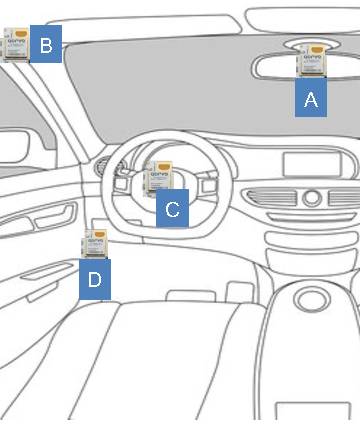
\includegraphics[height=3.5cm]{figures/anchor_placements.pdf}
%     % \caption{Anchor locations tested}
%     \label{fig:anchor_placements}
%   \end{subfigure}
%   \hfill
%   \begin{subfigure}[t]{0.66\linewidth}
%     \centering
%     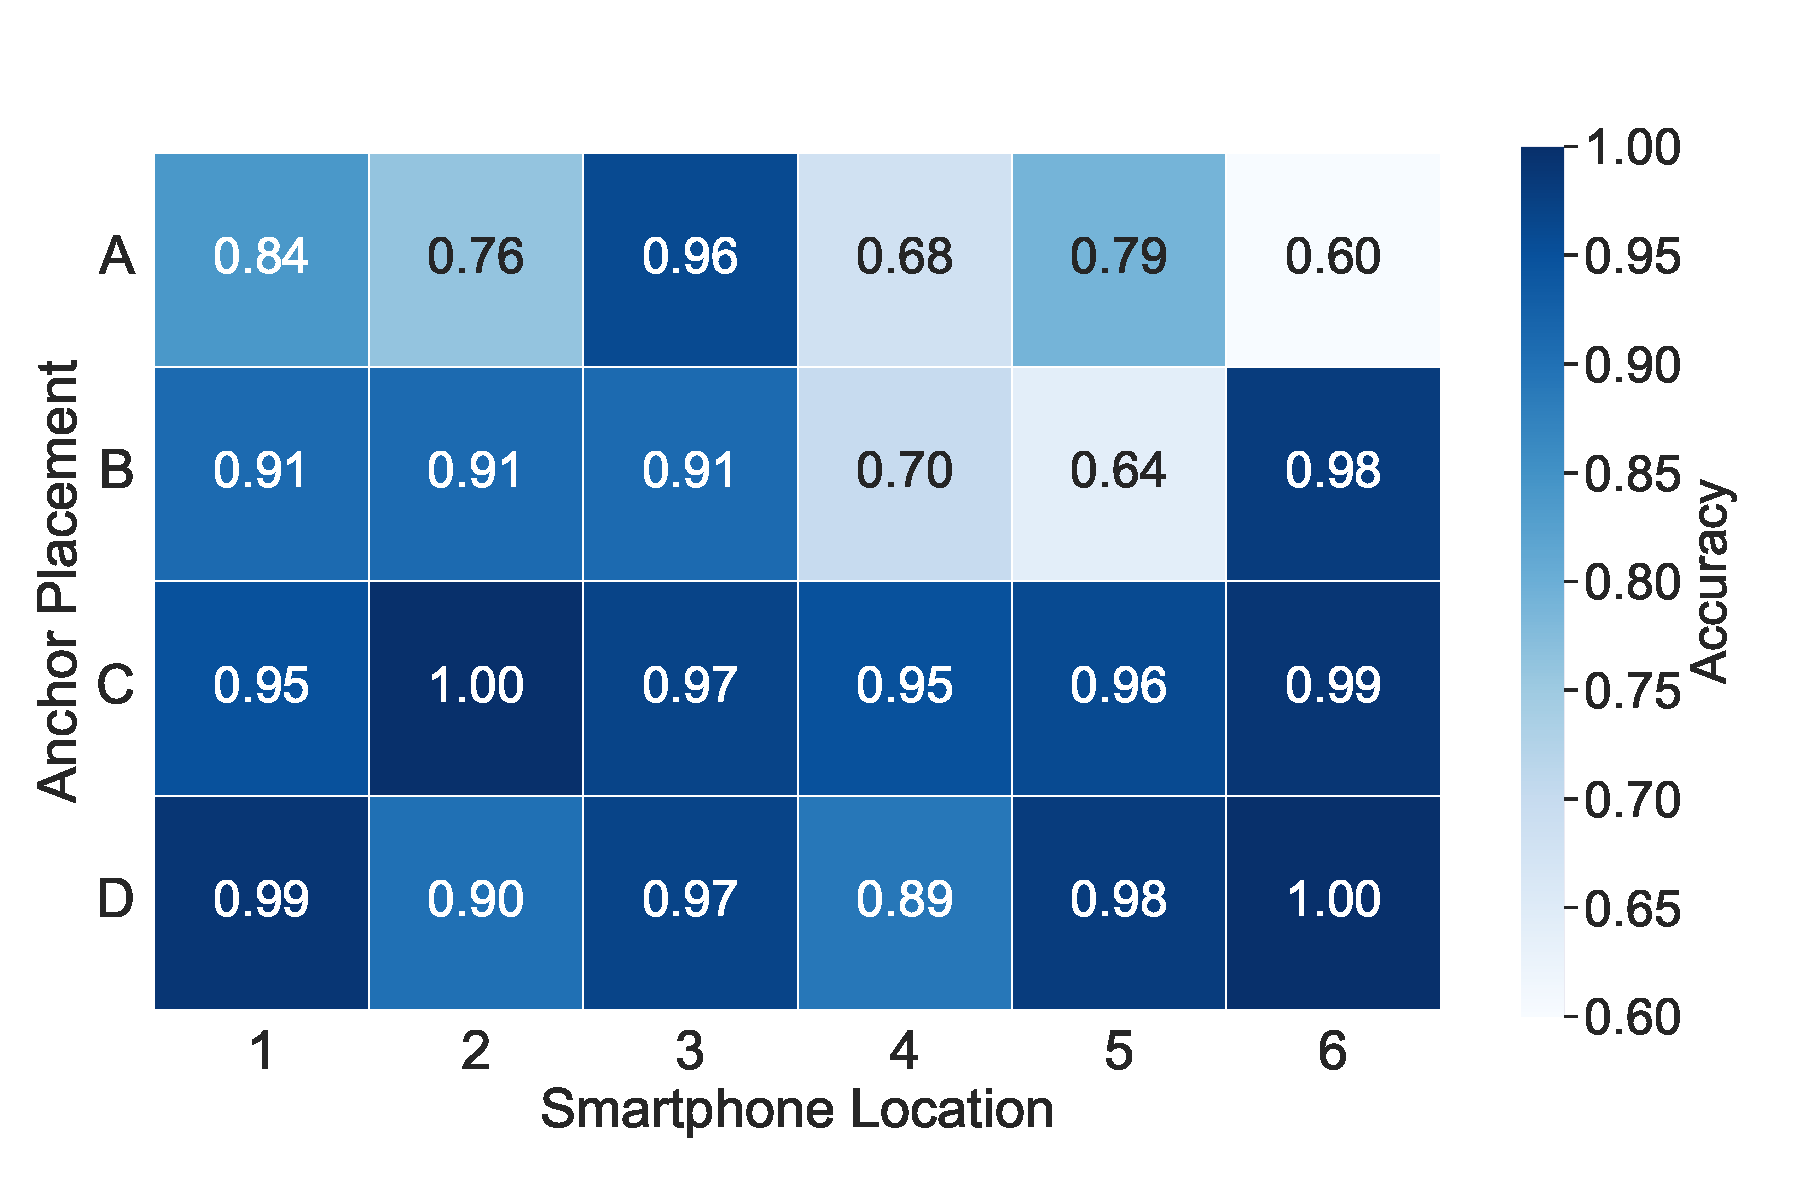
\includegraphics[height=3.5cm]{figures/anchor_placements_accuracy.pdf}
%     % \caption{Classification accuracy by placement}
%     \label{fig:anchor_placements_accuracy}
%   \end{subfigure}
%   \caption{Impact of anchor placement: (a) Anchor positions tested, (b) classification accuracy at each phone location.}
%   \label{fig:anchor_accuracy_combined}
% \end{figure}

\begin{figure}[t]
  \centering
  \begin{subfigure}[t]{0.44\linewidth}
    \centering
    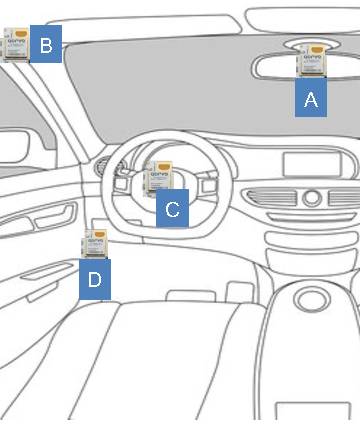
\includegraphics[height=\linewidth]{figures/anchor_placements.pdf}
    \caption{Anchor placements.}
    \label{fig:anchor_placements}
  \end{subfigure}
  \hfill
  \begin{subfigure}[t]{0.44\linewidth}
    \centering
    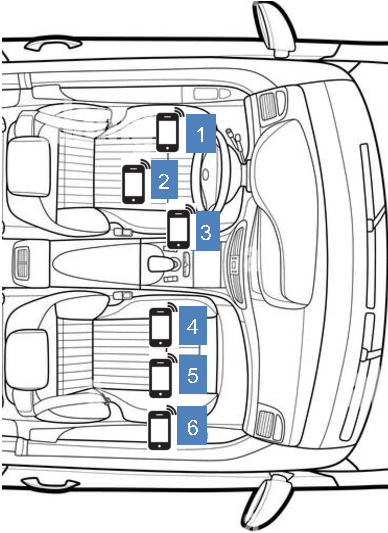
\includegraphics[height=\linewidth]{figures/smartphone_locations_narrow.pdf}
    \caption{Smartphone locations.}
    \label{fig:smartphone_locations}
  \end{subfigure}
  \vp
  \caption{Anchor and smartphone Locations.}
  \label{fig:placement_config}
  \vp
\end{figure}




\begin{figure}[t]
  \centering
  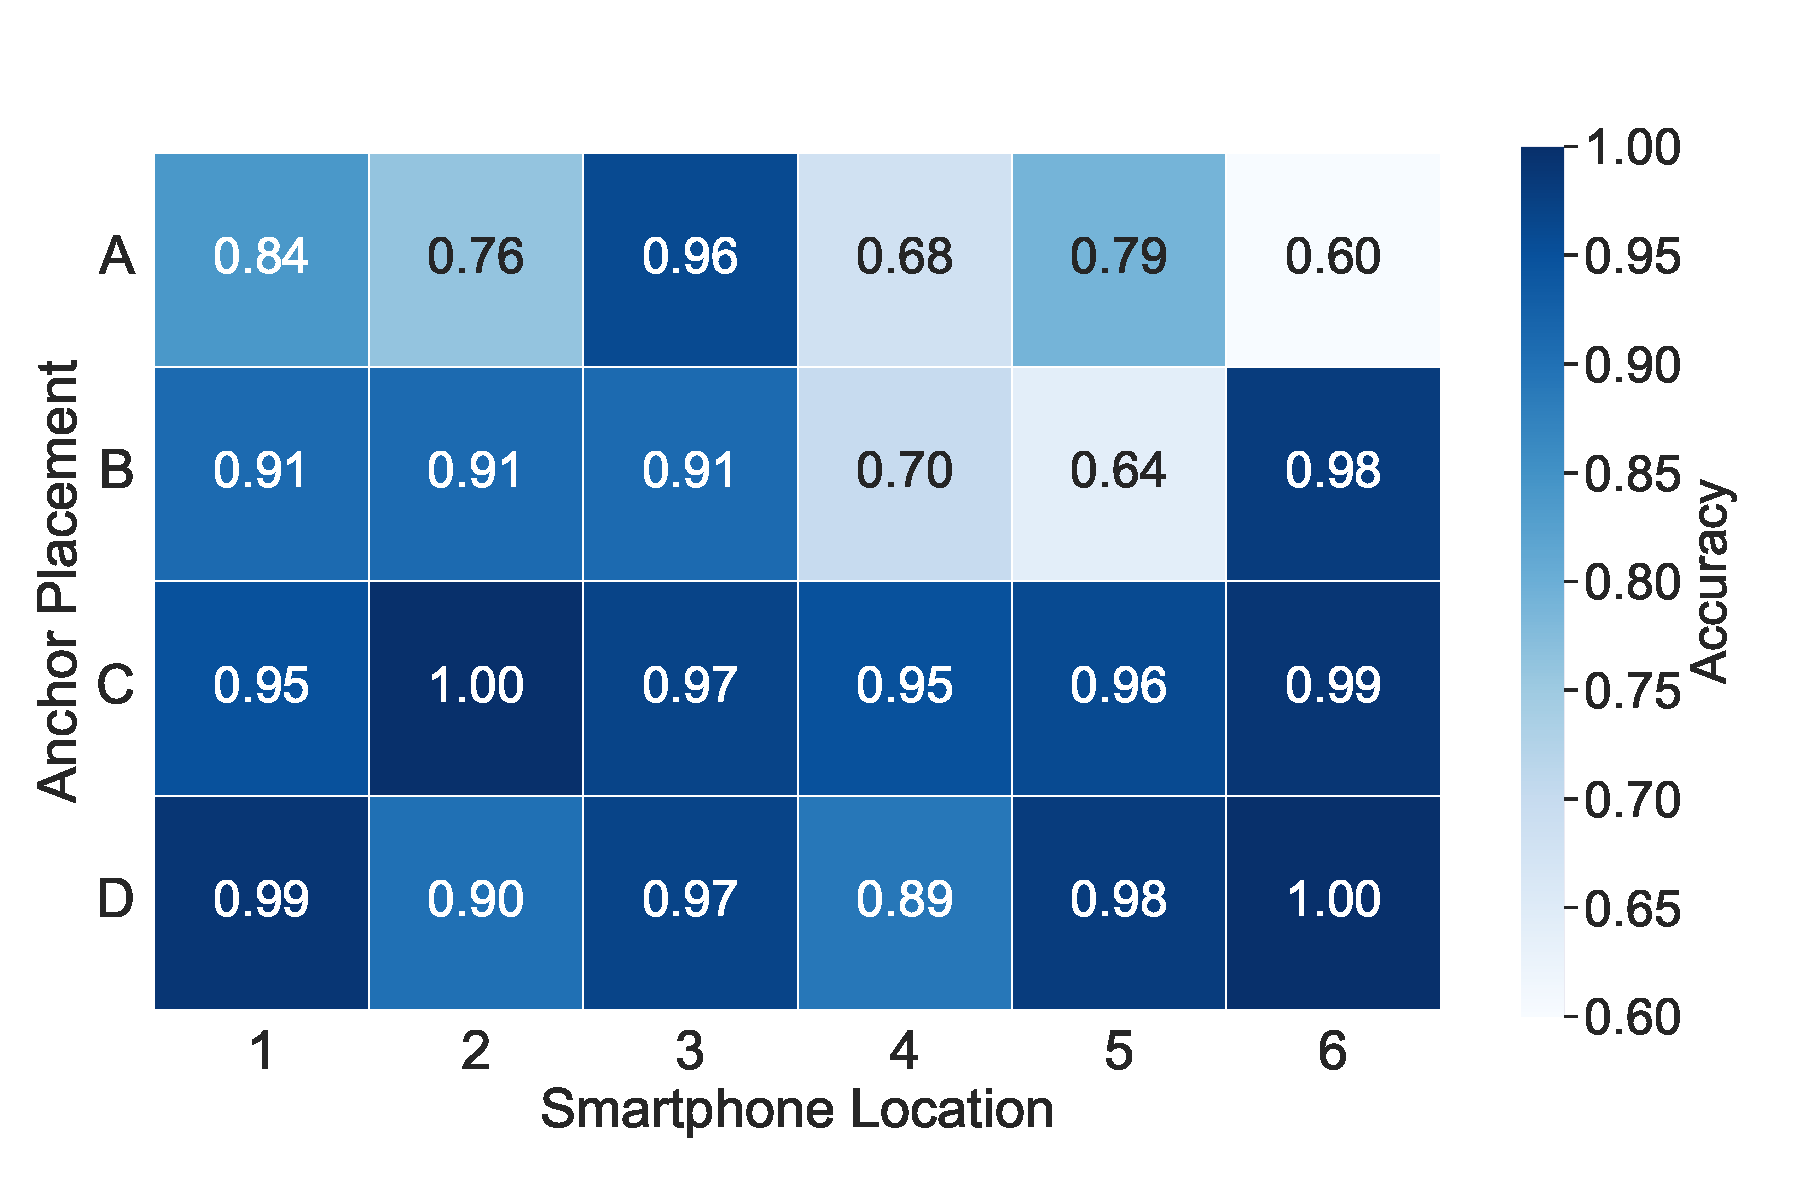
\includegraphics[width=0.75\linewidth,trim={0 1cm 0 2cm},clip]{figures/anchor_placements_accuracy.pdf}
  \vp
  \caption{Classification accuracy at each smartphone location across different anchor placements.}
  \label{fig:anchor_placements_accuracy}
  \vp
\end{figure}

Fig.~\ref{fig:anchor_placements_accuracy} shows the classification testing 
results with different anchor placement and smartphone locations.
%
When the anchor is placed at the rearview mirror, several driver- and 
passenger-side regions produce overlapping CIR and distance measurements, 
degrading classification accuracy, especially in the passenger left and driver 
right areas. 
%
To break this symmetry, we test relocating the anchor to the top of the
driver-side door. This placement introduces clear distance asymmetry between 
driver and passenger seats.
%
However, UWB ranging alone is unreliable in this environment due to in-cabin 
multipath effects, especially when multiple reflective surfaces (e.g., seats, 
windows, dash) lie close to the signal path. 
%
As shown in Fig.~\ref{fig:ranging_overlap}, this placement suffers from 
overlapping distance distributions across seat regions.
%
CIR features remain ambiguous in such configurations due to merged or
indistinct peaks, especially when the reflective paths from symmetric seat
regions remain geometrically similar (Fig.~\ref{fig:ambiguity_cir}).



To mitigate this, we explore anchor placements that simultaneously amplify 
asymmetries in both ranging and CIR profiles.
%
As shown in Fig.~\ref{fig:anchor_placements_accuracy}, positions, such as
the steering-wheel column and OBD-II port, show better performance than other positions as they introduce significant geometric 
differentiation across all front-row positions.
%
These placements shift the overlap region in ranging space to locations where 
CIR features remain distinguishable, enabling joint disambiguation.
%
For example, with the anchor mounted on the steering-wheel column, driver-left 
and passenger-right positions may have similar path lengths, but their CIRs differ 
substantially due to proximity to reflective surfaces like the dashboard 
or vehicle pillars.
%
As illustrated in Fig.~\ref{fig:steer_top_CIR}, CIR peaks shift based on local 
reflectors: when the smartphone is close to surfaces such as the door, 
the non-primary peaks appear earlier due to short 
reflection paths; when positioned near the cabin center, those peaks are
more delayed.

Our results show that anchor positions such as the steering wheel column and
OBD-II port provide more distinguishable propagation characteristics due to 
structural asymmetry. 
%
These placements jointly improve the separability of both CIR and distance 
features and serve as effective alternatives when design-time control is available.


\begin{figure}[t]
    \centering
    \includegraphics[width=0.8\linewidth]{figures/ranging_overlap.png}
    \vp
    \caption{Ranging results at two smartphone locations.}
    \label{fig:ranging_overlap}
    \vp
\end{figure}

\begin{figure}[t]
    \centering
    \includegraphics[width=0.7\linewidth]{figures/steer_top_CIR.png}
    \vp
    \caption{CIR distinguishes 2 overlapped-ranging locations.}
    \label{fig:steer_top_CIR}
    \vp
\end{figure}

\subsubsection{Shielding UWB Anchor} In scenarios where \name~is retrofitted into 
existing vehicles with built-in UWB-based keyless entry systems, relocating the 
anchor is impractical.
%
FCC filings show that some manufacturers install UWB transceivers along the 
vehicle’s centerline, typically near the rearview mirror or rear brake light, 
to maximize in-cabin and exterior coverage \cite{fcc_audi_uwbtrx22_2021, 
fcc_bmw_fbd5_2021}.
%
However, this centralized placement creates geometric symmetry between driver
and passenger seats, leading to overlapping CIR and ranging features that limit 
localization precision.

To address this challenge without modifying vehicle hardware,
we propose a lightweight, non-invasive solution: attaching a small metal shield 
near the UWB anchor antenna to induce directional asymmetry in signal propagation.
%
Inspired by RF metasurface principles, the shield is designed to attenuate 
signals toward one side of the cabin while enhancing reflections toward the
other, improving separability in multipath signal characteristics.

\textbf{Shield’s Effect on Signal Propagation}:
Metals such as aluminum are effective at attenuating and reflecting RF signals
due to their high conductivity \cite{shakya2024wideband, iya2011ultra}.
%
The curvature of the reflective surface also influences propagation directionality, 
a concept leveraged in prior beam-shaping systems \cite{xiong2017customizing, han2017enhancing}.

To evaluate this effect, we placed a half ping-pong ball (radius 20 mm) coated
with aluminum foil adjacent to the driver-facing side of the UWB antenna.
%
We compare signal features with and without the shield across six front-row 
locations (Fig.~\ref{fig:smartphone_locations}) by collecting $1,000$ 
real-world CIRs and RSSIs at each location. The RSSI is computed by the hardware as a function of the CIR power \cite{Dw3000}.

The results show clear directional asymmetry. 
% As shown in 
% Fig.~\ref{fig:rssi_shielded_map}, signals toward the blocked (driver) side are 
% attenuated, while those toward the open (passenger) side are enhanced via 
% reflection. As shown in Fig.~\ref{fig:rssi_shielded_map}, driver-side RSSI 
% values are reduced by 3–5 dB on average, while reflections toward the 
% open (passenger) side are enhanced.
As shown in Fig.~\ref{fig:rssi_shielded_map}, signals toward the blocked (driver) side are attenuated (RSSI $\approx$3 dBm lower on average), while reflections toward the open (passenger) side are enhanced (RSSI  $\approx$4 dBm higher on average).
%
% CIR profiles also shift accordingly: early peaks are suppressed on the blocked 
% side as the direct path is attenuated, while late peaks on the open side
% are elongated due to additional indirect paths.
CIR profiles also shift accordingly: on the blocked side, early peaks are 
attenuated as the direct path is obstructed by the shield; on the open side, 
late peaks are suppressed due to the lack of energy reflected back from the 
now-blocked region (Figs.~\ref{fig:cir_shielded_example} and~\ref{fig:shield_signal_propagation}).

To quantify these effects, we extract two features: RSSI and late energy ratio, 
the proportion of CIR energy arriving more than 1,000 samples (4.7m) after the 
first peak.
%
As shown in Fig.~\ref{fig:shield_boxplots_features}, both features exhibit 
strong side-dependent separation.
%
However, intra-seat variation caused by phone orientation, anchor distance, 
and environmental reflections introduces overlap. 
%
Even within a single location, RSSI can fluctuate by $\pm3$ dBm, and tail
energy ratio can vary widely, potentially degrading classification performance.

\begin{figure}[t]
    \centering
    \includegraphics[height=0.46\linewidth]{figures/rssi_shielded_map.png}
    \vp
    \caption{Average RSSI values  w/ and w/o shield (dBm).}
    \vspace{-10pt}
    \label{fig:rssi_shielded_map}
    \vp 
\end{figure}

% \begin{figure}
%     \centering
%     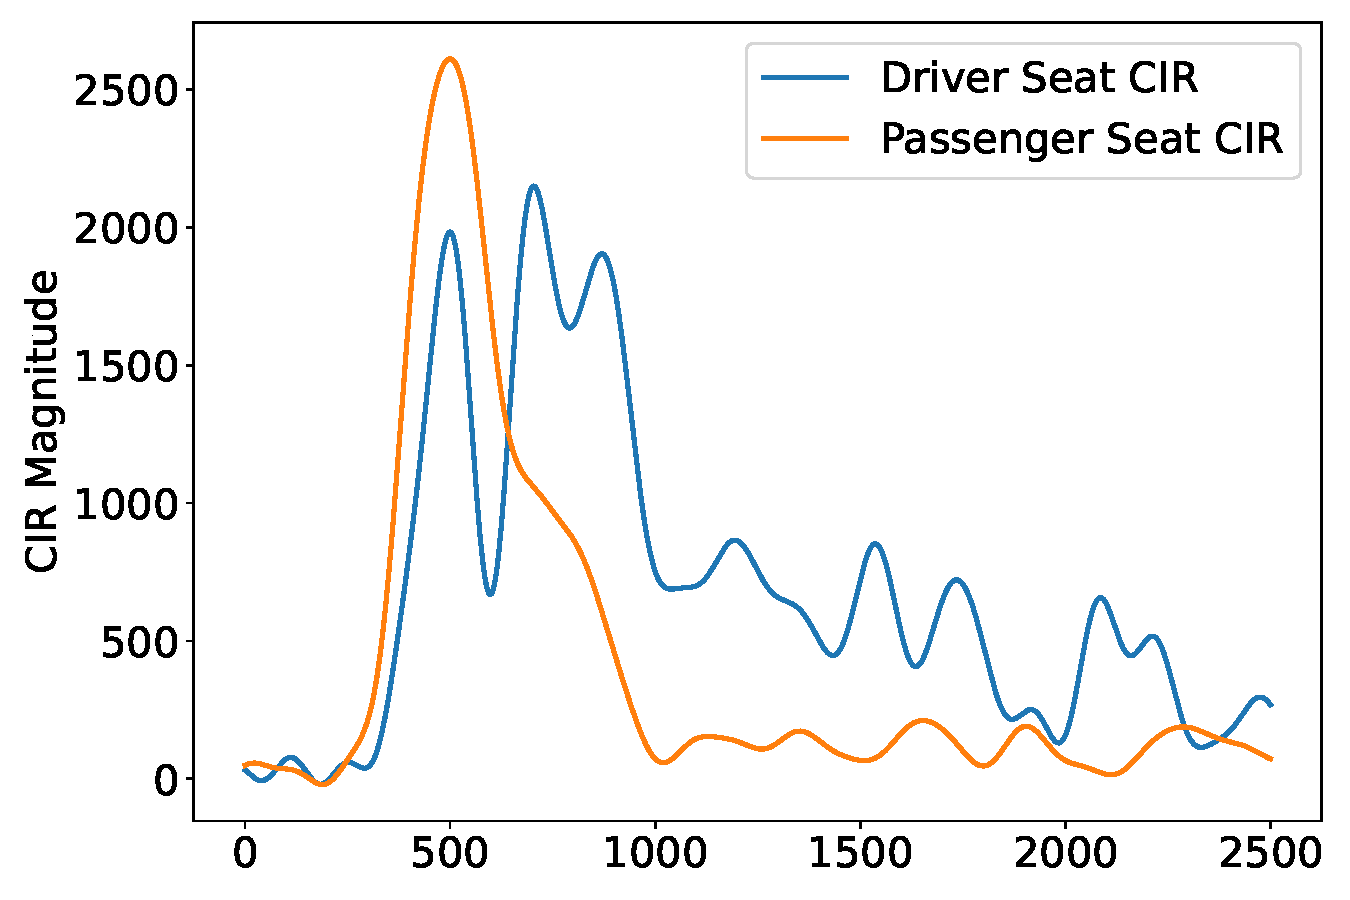
\includegraphics[width=0.9\linewidth]{figures/cir_shielded_example.pdf}
%     \caption{CIRs from driver and passenger seat when shield is placed}
%     \label{fig:cir_shielded_example}
% \end{figure}

% \begin{figure}
%     \centering
%     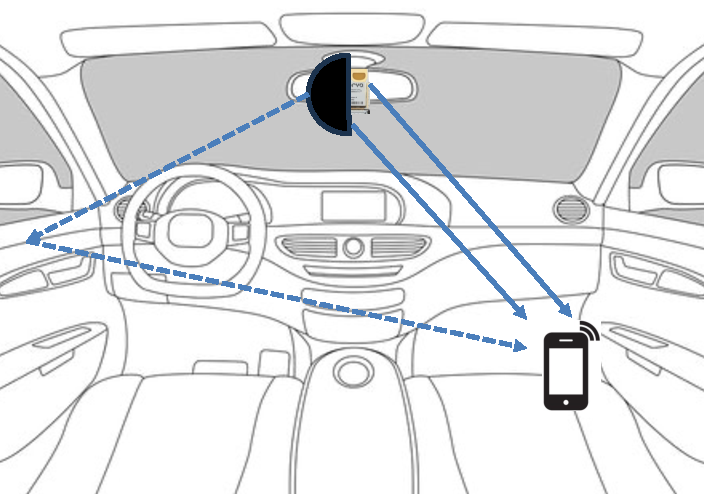
\includegraphics[width=0.9\linewidth]{figures/shield_signal_propagation.png}
%     \caption{Signal propagation path to passenger when shield is placed}
%     \label{fig:shield_signal_propagation}
% \end{figure}

\begin{figure}[t]
  \centering
  \begin{subfigure}[t]{0.46\linewidth}
    \centering
    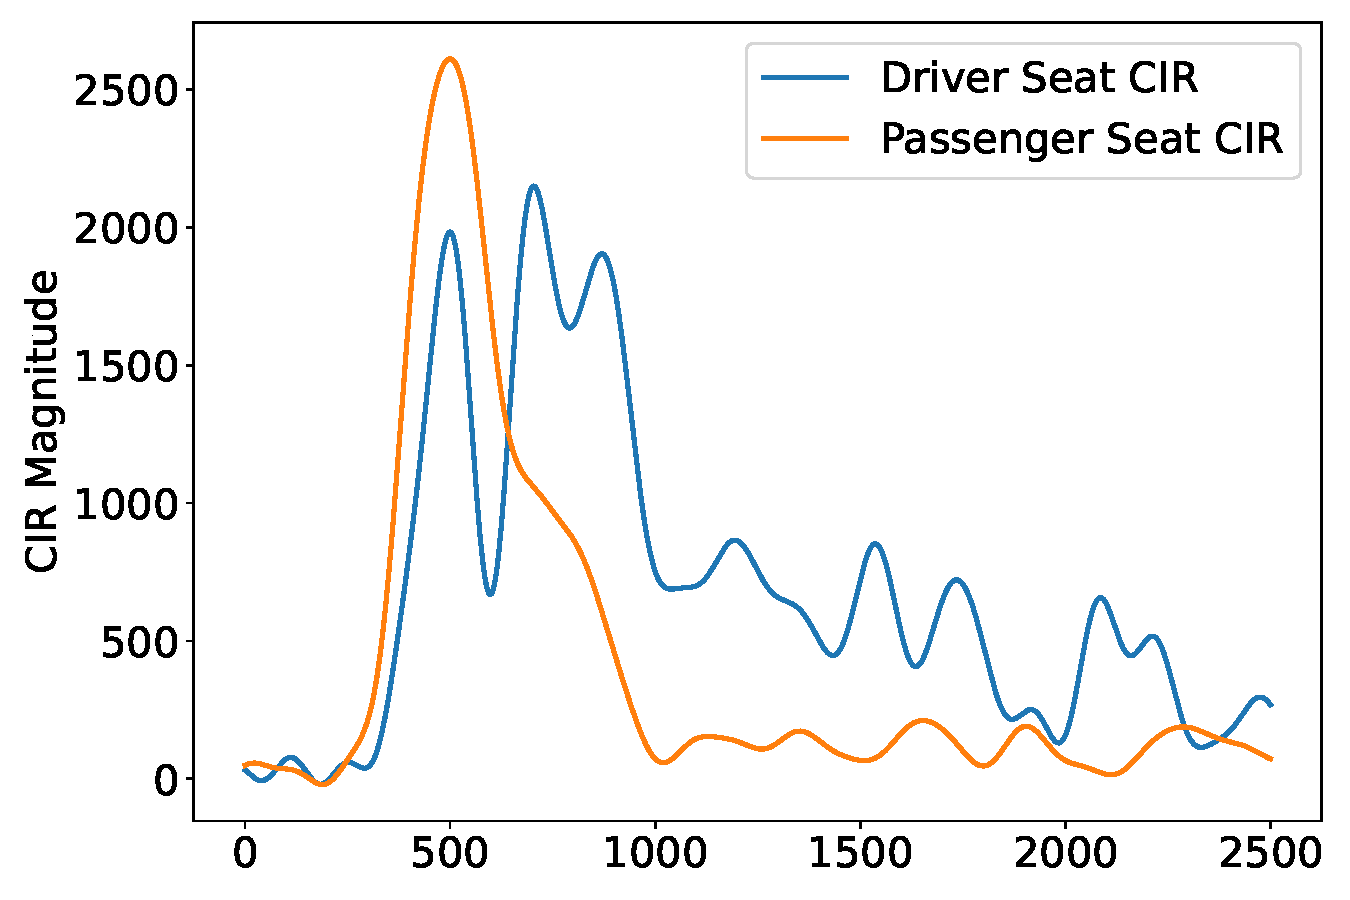
\includegraphics[width=\linewidth]{figures/cir_shielded_example.pdf}
    \caption{CIRs from driver and passenger seat with directional shield.}
    \label{fig:cir_shielded_example}
  \end{subfigure}
  \hfill
  \begin{subfigure}[t]{0.46\linewidth}
    \centering
    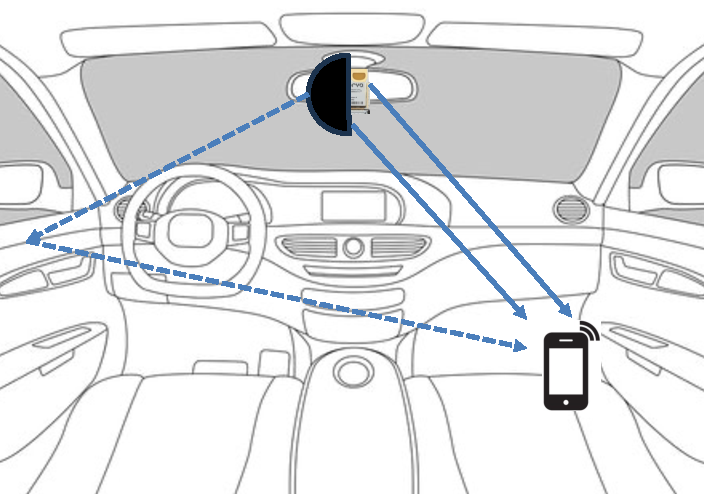
\includegraphics[width=\linewidth]{figures/shield_signal_propagation.pdf}
    \caption{Shield enhances signal to passenger while attenuating signal to driver side.}
    \label{fig:shield_signal_propagation}
  \end{subfigure}
  \vp
  \caption{Impact of directional shielding on CIR and propagation path.}
  \label{fig:fig_shielded_combined}
  \vp
\end{figure}

\begin{figure}[h]
    \centering
    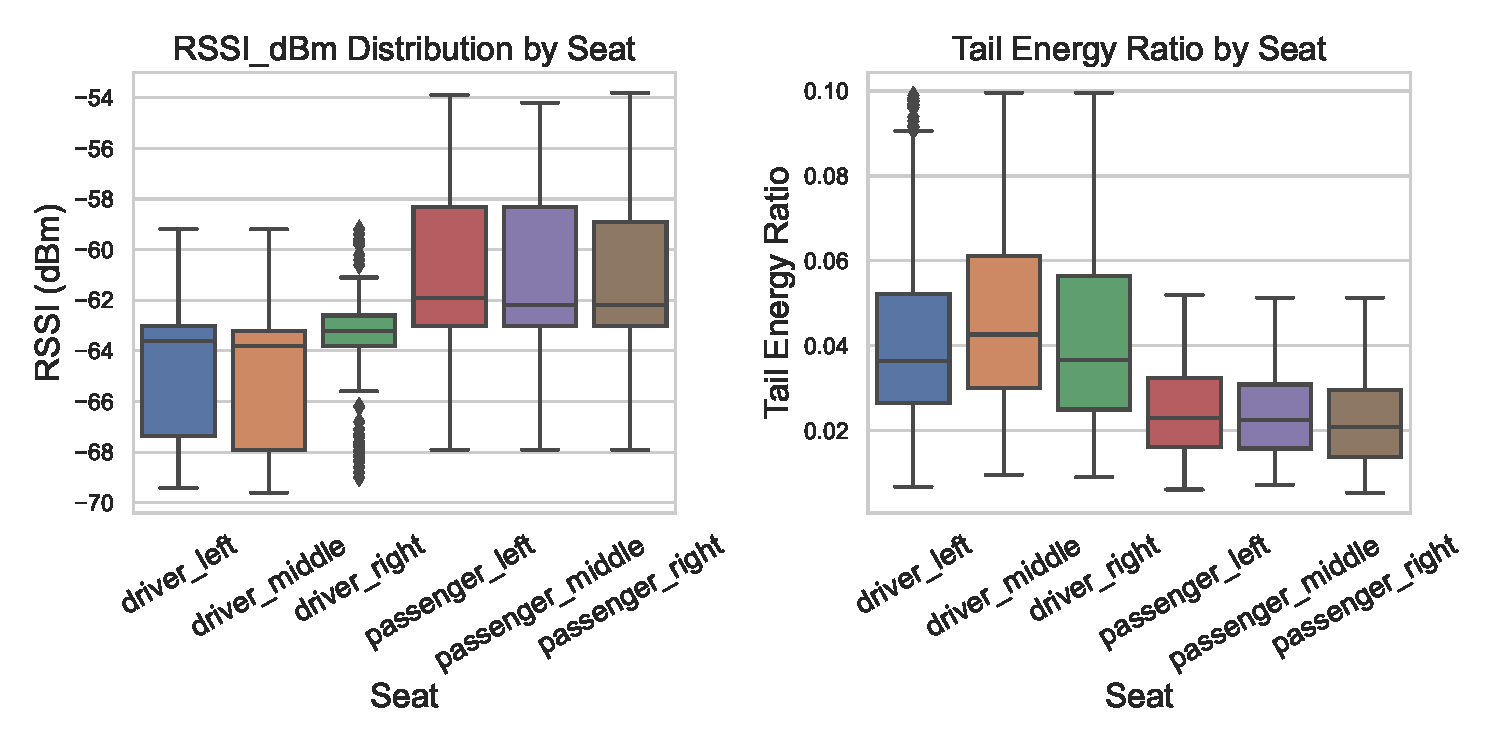
\includegraphics[height=0.46\linewidth]{figures/shield_features_distribution.pdf}
    \vp
    \caption{RSSI and Late Energy Ratio at 6 front row locations.}
    \label{fig:shield_boxplots_features}
    \vp
\end{figure}


These findings raise a key design question: \textit{How can we design a metal 
shield that consistently produces sufficient signal feature separation across all 
front-row locations to enable robust driver-passenger smartphone localization?}

\textbf{Shield Design}:
%
To answer this, the shield must satisfy two criteria: (i) induce sufficient signal 
feature separation across all seat positions, and (ii) minimize the transitional 
zone, or borderline region, where signals diffraction or partial reflection blurs 
classification boundaries.
%
We explore variations in shield shape and size to achieve these objectives. 

Because UWB antennas are omnidirectional, the shield must partially enclose the 
antenna to block propagation in a specific direction.
%
To support driver-passenger classification, either side can be attenuated;
in our implementation, we focus on shielding the driver side.
%
We prototype multiple 3D-printed shield geometries, including hemispheres, 
half-cylinders, and half-open rectangles, each wrapped in aluminum foil, a 
lightweight and effective RF reflective material \cite{xiong2017customizing,han2017enhancing}.
%
These shields are mounted near the most typical UWB anchor location, i.e., 
at the rearview mirror. 
%
The design principles can be generalized to other anchor locations.


\begin{figure}[]
    \centering
    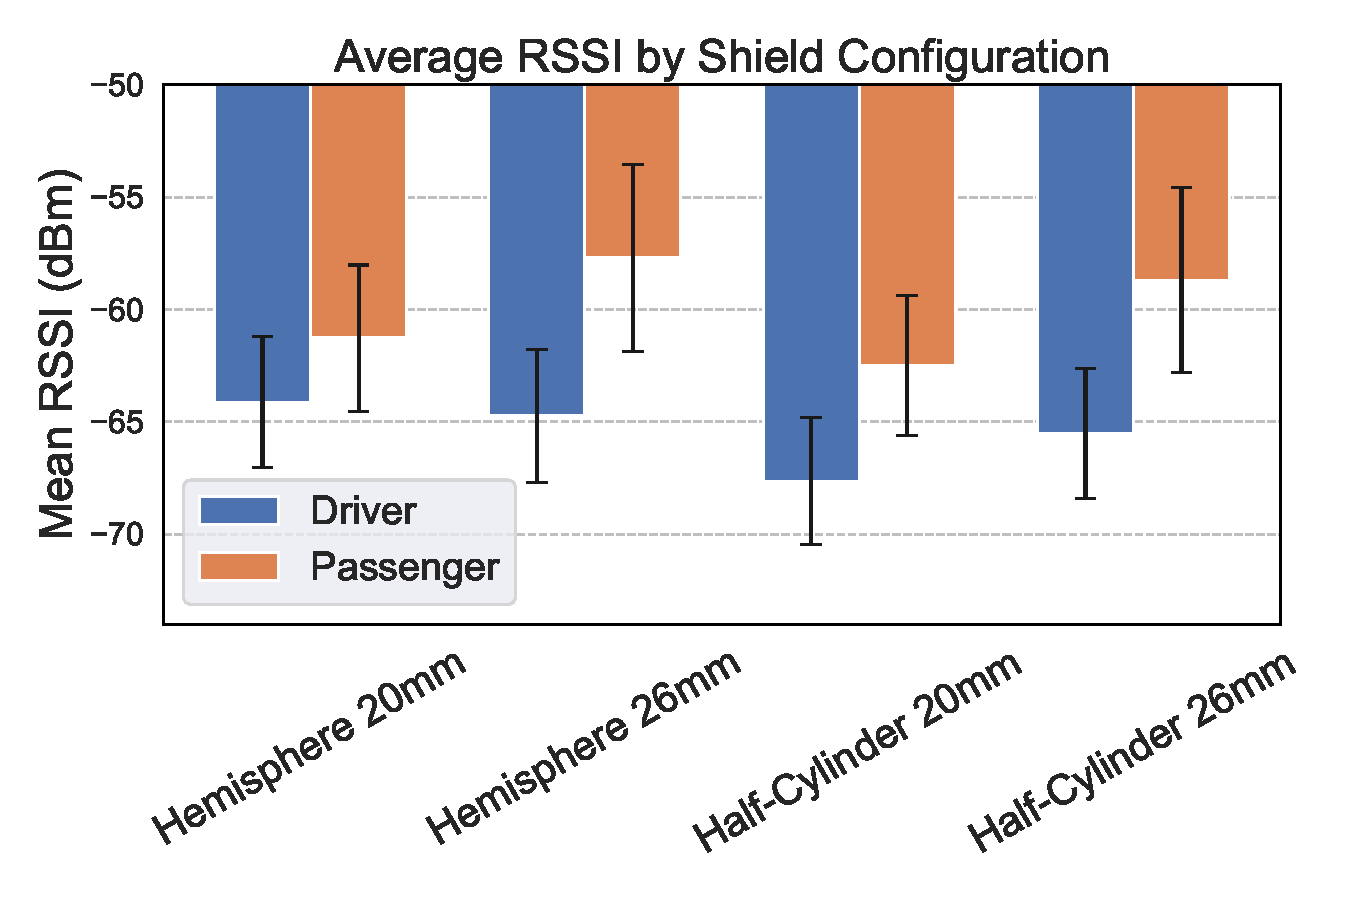
\includegraphics[width=0.77\linewidth]{figures/rssi_shield_size.pdf}
    \vp
    \caption{Driver and passenger RSSI values of different shield sizes.}
    \label{fig:rssi_shield_size}
    \vspace{-15pt}
\end{figure}
\textit{Shield Size}:
Larger shields reflect and block more radiated energy, producing stronger asymmetry.
%
However, they must remain compact and visually unobtrusive, ideally fitting
within the transceiver’s form factor to blend into the vehicle interior.
%
We tested hemisphere and half-cylinder shields with radii of $20$ mm and $26$ mm 
($52$ mm height for half-cylinders), based on the $28$ × $20$ mm footprint of 
the UWB module.
%
For each size, we measure RSSI at all driver- and passenger-side seat locations. 
%
As shown in Fig.~\ref{fig:rssi_shield_size}, larger shields yielded greater 
RSSI separation and more separation between two sides, resulting in higher 
classification accuracy (see Fig.~\ref{fig:shield_accuracy}).



\textit{Shield Shape}:
%
Since the UWB antenna is omnidirectional, partial shielding creates a borderline 
region, a transitional angular zone between the blocked and open sides.
%
In this region, phones may receive diffracted signals or weakened reflections, 
resulting in ambiguous RSSI and CIR features for localization 
(Fig.~\ref{fig:diffraction_shield_table}).
%
To quantify the extent of this region, we conducted controlled experiments with
the phone placed along a circular arc (–25° to +25° in 5° increments) centered
on the UWB antenna.
%
At each angle, we measured signal features and evaluated classification accuracy 
using a pre-trained model. We then identified the angular range where 
accuracy dropped below 80\%, marking it as the borderline region.
%
We repeated this for three shield shapes: hemisphere, half-cylinder, and 
half-open rectangle. 
%
As shown in Fig.~\ref{fig:diffraction_shield_table}, the half-cylinder has 
the narrowest ambiguity zone, suggesting it best suppresses diffraction while 
maintaining signal reflection strength.

\begin{figure}[t]
  \centering
  % 1. Added [b] to perfectly align both captions horizontally
  \begin{minipage}[b]{0.37\linewidth}
    \centering
    % 2. Added trim and clip to cut out the invisible bottom margin in the PDF
    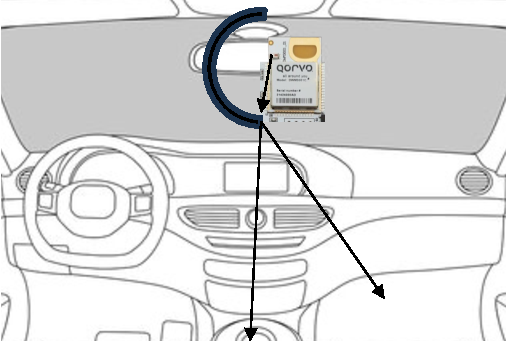
\includegraphics[width=0.88\linewidth]{figures/shape_diffraction_short.pdf}
    \caption*{(a) Sector ambiguity due to diffraction.}
  \end{minipage}%
   \hfill
  \begin{minipage}[b]{0.55\linewidth}
  \centering
  \small
  \begin{tabular}{|c|c|}
    \hline
    \makecell{\textbf{Shield} \\ \textbf{Shape}} & 
    \makecell{\textbf{Borderline} \\ \textbf{Angular Span}} \\ \hline
    Hemisphere & $20^\circ \pm 5^\circ$ \\
    \hline
    \makecell{Half-Open \\ Rectangle} & $20^\circ \pm 5^\circ$ \\
    \hline
    Half-Cylinder & $15^\circ \pm 5^\circ$ \\ \hline
  \end{tabular}
  % You may be able to remove this \vspace now that the bottoms are aligned!
  \vspace{-10pt} 
  \caption*{(b) Angular spans under different shield shapes.}
\end{minipage}
  \vp
  \caption{Measured diffraction effects caused by shielding.}
  \label{fig:diffraction_shield_table}
  \vspace{-1.5em}
\end{figure}





% \begin{figure}
%     \centering
%     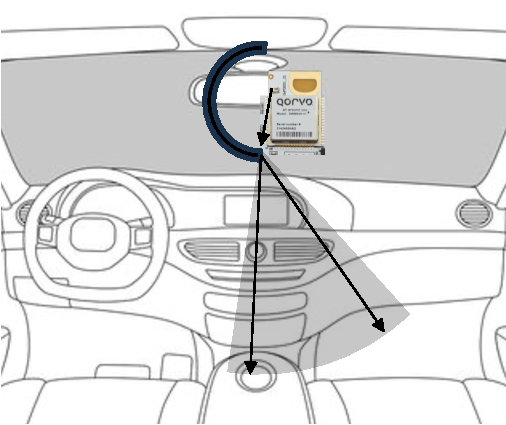
\includegraphics[width=0.8\linewidth]{figures/shape_diffraction.pdf}
%     \caption{Diffraction leads to a sector region of ambiguity }
%     \label{fig:shape_diffraction}
% \end{figure}

% \begin{table}[t]
% \centering
% \caption{Measured angular span of borderline region of uncertainty of $\pm$5°}
% \label{tab:borderline_region}
% \begin{tabular}{|l|c|}
% \hline
% \textbf{Shield Shape} & \textbf{Borderline Angular Span} \\
% \hline
% Hemisphere            & 20° $\pm$ 5° \\
% Half-Open Rectangle   & 20° $\pm$ 5° \\
% Half-Cylinder         & 15° $\pm$ 5° \\
% \hline
% \end{tabular}
% \end{table}

\textit{End-to-end Localization with Shield}:
To assess how each shield design supports robust end-to-end seat-level 
classification, we evaluate classification accuracy across six front-row 
smartphone locations (Fig.~\ref{fig:smartphone_locations}). 
%
We select four representative designs based on shield size and shape 
insights: the hemisphere ($r=$ 20mm) as the baseline, hemisphere
($r=$ 26mm) to study effect of shield size, cylinder ($r=$ 26mm) for optimal 
performance, and a half-open rectangle (26mm × 52mm).
%
For each shield configuration, we collected approximately 1,200 samples per smartphone location, spanning 6 locations shown 
in (Fig.~\ref{fig:smartphone_locations}). The data was randomly split 
into 80\% for training and 20\% for testing. Besides the features
in Table \ref{tab:CIR_features}, we include RSSI and features that reflect late peaks (Table \ref{tab:Shield_features}).

We apply temporal smoothing by averaging the additional features (Table \ref{tab:Shield_features}) in over a short window 
of 7 frames (1.4 seconds). Both RSSI and late CIR peaks exhibit high 
frame-to-frame variability (Fig.~\ref{fig:shield_boxplots_features}) as the late 
peaks are the result of distant, weaker multipath components that more susceptible 
to fluctuations caused by small movements of the phone. Smoothing over multiple 
frames helps mitigate such noise and produces more consistent inputs for the 
classifier. Unlike the steering-top anchor configuration, peak tracking is not applied in the shielded setup, as late-peak-based features do not benefit meaningfully from inter-frame peak consistency. We train 
a classifier (same model as in Section \ref{sec:system::localization}) to 
distinguish between driver-side and passenger-side locations. 
\begin{table}[t]
\caption{Additional features for shielded anchor setup.}
\label{tab:Shield_features}
\vp\small
\begin{tabular}{|l|}
\hline
\textbf{Features description }                                      \\ \hline
Received signal strength indicator               \\ \hline
Ratio of energy 1000 indices after first peak to total energy                 \\ \hline
Number of CIR peaks 1000 indices after first peak. \\ \hline
Position of the latest detected peak in the CIR.   \\ \hline
\end{tabular}
\vspace{-2.2em}
\end{table}

The hemisphere ($r = 20 $mm) shows sub-90\% accuracy at multiple positions, 
primarily due to the limited feature separation between the blocked and open sides. 
Both the hemisphere ($r = 26 $mm) and the half-open rectangle perform well 
when the phone is far from the car’s midline but degrade at edge positions near 
the center, where signal features overlap due to diffraction and partial occlusion. 
%
In contrast, the cylinder ($r = 26 $mm) maintains $>97\%$ accuracy at all 6
positions, confirming its small borderline ambiguity region and large enough 
feature separation.
%
Thus, we adopt the 26 mm half-cylinder as our default shield design.

\begin{figure}[t]
    \centering
    \vspace{10pt}
    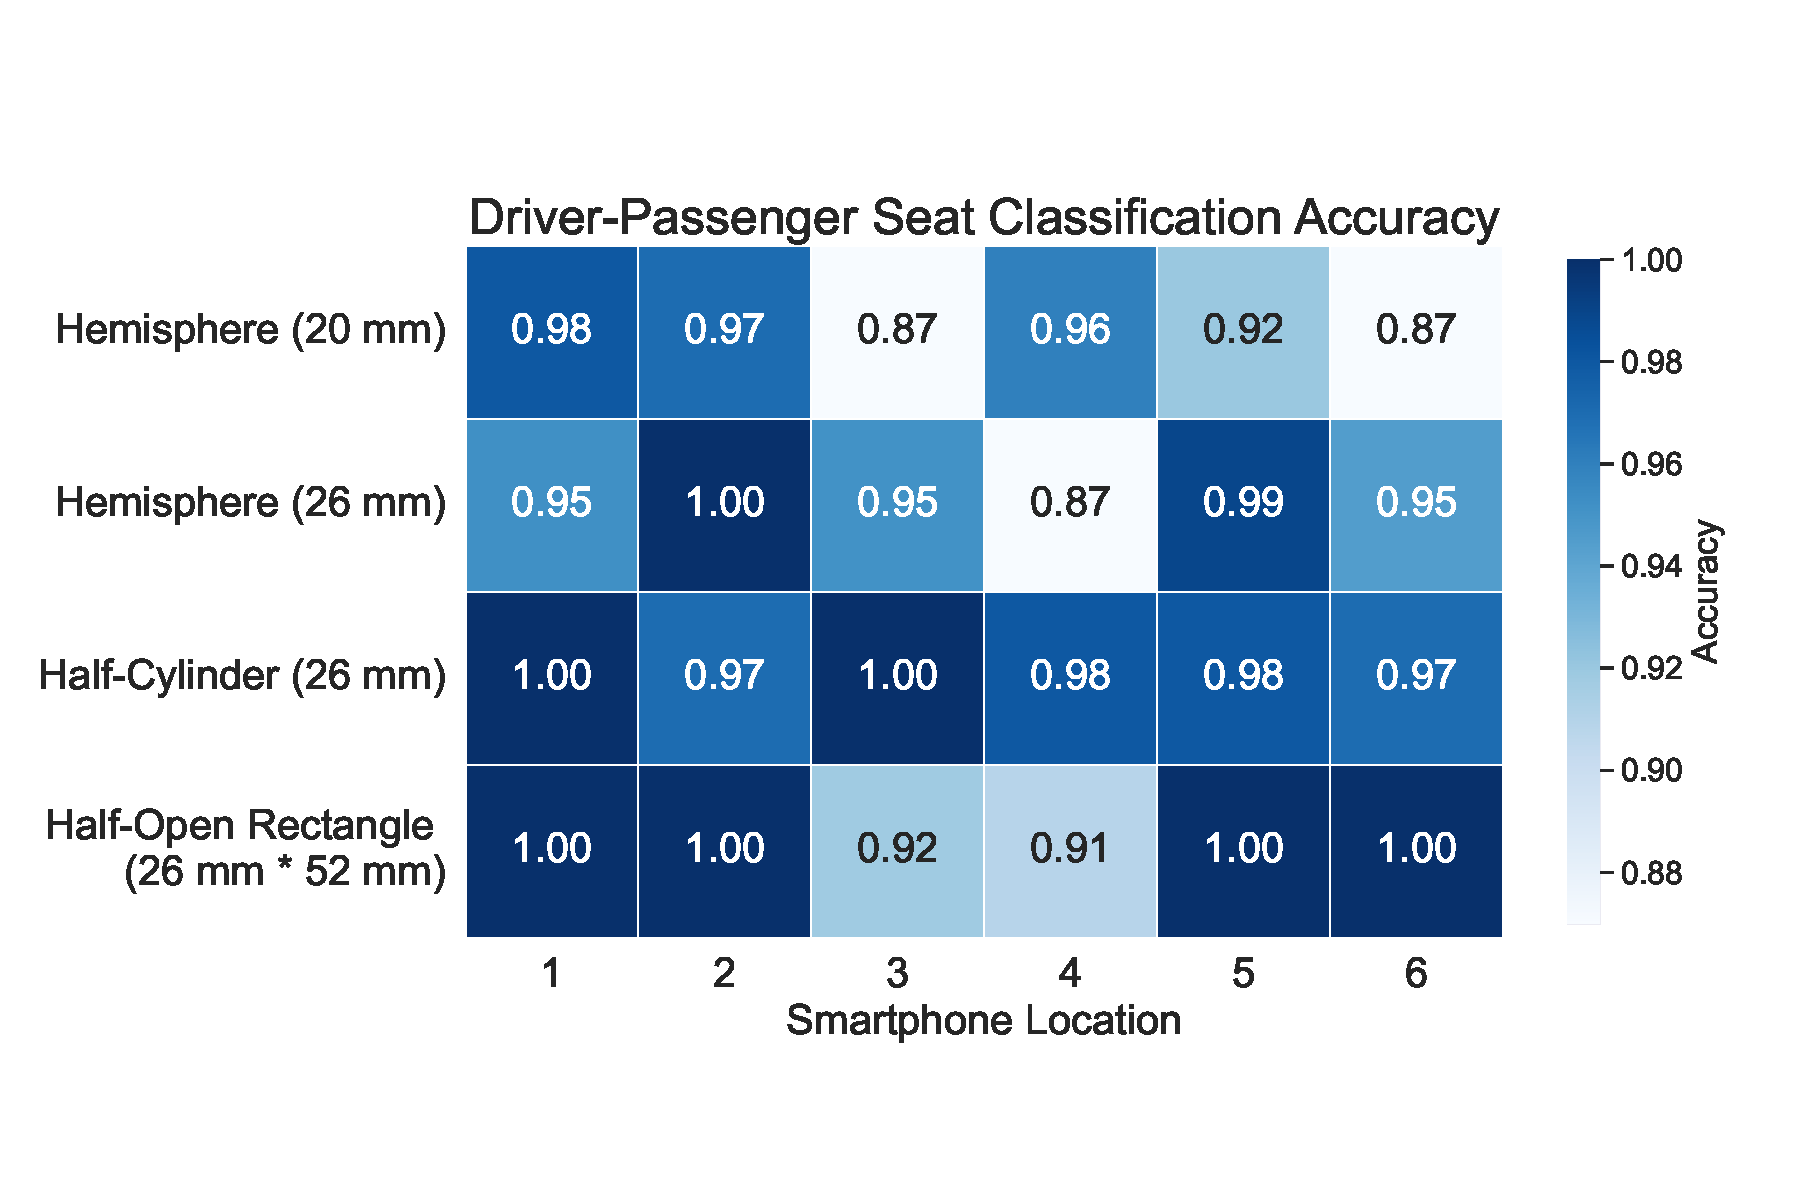
\includegraphics[width=0.9\linewidth,trim={0 2.5cm 0 3cm},clip]{figures/shield_accuracy.pdf}
    \vp
    \caption{Classification accuracy at six front row locations for four shield designs.}
    \label{fig:shield_accuracy}
    \vp
\end{figure}

\textbf{Guaranteeing the normal usage of UWB anchor}:
The internal UWB transceiver is primarily designed for vehicle access control 
applications such as keyless entry \cite{fcc_bmw_fbd5_2021, fcc_audi_uwbtrx22_2021, Ultra-WidebandCCC}.
%
To ensure that our shielding design does not interfere with this functionality,
we tested UWB signal coverage by moving a smartphone within a 1-meter radius 
around the vehicle.
%
% We found that even on the shielded side, the smartphone was still able to perform accurate ranging with the in-vehicle UWB transceiver because of rich multipath propagation.
Even on the shielded side, the phone was able to maintain UWB connectivity and 
initiate ranging exchanges with the in-vehicle transceiver.
%
These results confirm that the proposed shield does not compromise the 
original functionality of the keyless entry system.

% \section{System Design}
% \label{sec:design}

% \subsection{Overview}
% We first give an overview of \name\  which is designed to localize smartphones 
% within a vehicle using a single in-cabin UWB anchor. 
% It consists of four main components: motion-triggered activation, 
% UWB ranging, CIR signal processing, and classification.

% When the smartphone enters a vehicle (detected through built-in smartphone OS 
% functionality), it begins monitoring IMU signals using a sliding time window. 
% If the system detects a cross-seat movement, it initiates UWB two-way ranging 
% with the anchor. For each ranging message exchange, the anchor transmits 
% distance measurements and CIR data to the smartphone. The phone performs 
% CIR processing in real time by tracking peaks across CIRs. 
% Once the CIR stabilizes, peak-based features are extracted, and then seat-level 
% classification is performed. 
% In case of multiple active smartphones, \name\ ensures each phone to access 
% the anchor in a round-robin fashion. 

% \begin{figure*}[htbp]
%     \centering
%     \includegraphics[width=\textwidth]{figures/system_design.png}
%     \caption{The workflow of \name's in-vehicle smartphone localization.}
%     \label{fig:system_design}
% \end{figure*}


% \subsection{Triggering of UWB Ranging}

% Out of the related works on in-vehicle smartphone localization, only \cite{chen2022vehicle} considered conditional triggering of localization. However, 

% \input{OLD/system}

\begin{figure}[t]
  \centering
  \begin{subfigure}[t]{0.22\textwidth}
    \centering
    \includegraphics[height=3cm]{figures/steering_top_anchor.png}
    \caption{Anchor on top of steering column.}
    \label{fig:steer_top_anchor}
  \end{subfigure}
  \hspace{10pt}
  \begin{subfigure}[t]{0.22\textwidth}
    \centering
    \includegraphics[height=3cm]{figures/shielded_anchor.png}
    \caption{Anchor next to rearview mirror with a shield attached.}
    \label{fig:rear_mirror}
  \end{subfigure}
\vp
\caption{Prototypes of two proposed anchor setups.}
  \label{fig:anchorimplementation}
  \vspace{-2em}
\end{figure}

\section{Evaluation}
\label{sec:evaluation}

\subsection{Experimentation Methodology}
\label{sec:evaluation:methodology}
\textbf{Phones and Cars Used.} While recent smartphones are equipped with UWB 
chips, their operating systems restrict access to low-level APIs necessary for capturing raw CIR data \cite{zhang2023embracing}.
%
Additionally, the UWB module integrated into a vehicle’s keyless entry system 
is controlled via the in-vehicle CAN bus, making it inaccessible for the 
continuous, large-scale data collection required by our experiments.
%
Thus, we use two DWM3001CDK UWB development kits, one is fixed inside the 
vehicle as the anchor, and the other is connected to a Samsung Galaxy 
S21 Ultra, emulating the smartphone’s UWB module.
%
Our evaluation spans three different vehicles: a BMW 3 Series \edited{(compact sedan)}, a Honda Accord \edited{(mid-size sedan)}, and a Honda CR-V \edited{(SUV)}.

\textbf{Implementation.} We develop an Android app for \name. 
It continuously monitors IMU data to detect cross-seat phone movements.
Upon movement detection, it triggers UWB ranging and, captures and processes 
CIR data to infer the phone’s seat-level location in real time.
%
We evaluate two anchor deployment configurations separately: 
(1) steering-top
anchor: the UWB anchor is placed at the identified optimal location, i.e., above
the steering wheel (Fig.~\ref{fig:anchorimplementation} (a)); (2) shielded
anchor: the anchor is positioned next to the rearview mirror with 
a custom half-cylinder RF shield attached (Fig.~\ref{fig:anchorimplementation} (b)).
%
For both configurations, we collect approximately 12,000 CIR and ranging 
samples from the smartphone across 8 predefined regions, including those in Fig.~\ref{fig:anchor_placements_accuracy} and two rear seat locations (left side and right side).
%
Each sample is labeled as corresponding to either the driver or passenger seat, 
and a lightweight Random Forest classifier is trained to distinguish between 
the two.

% \begin{figure}[t]
%     \centering
%     \includegraphics[width=0.7\linewidth]{figures/eval_smartphone_locations.png}
%     \vp\caption{Smartphone locations tested.}
%     \label{fig:eval_locations}
%     \vp
% \end{figure}

\textbf{Localization Accuracy.}
We first evaluate the localization accuracy of the trained model across 
different smartphone locations. At each of these 8 predefined regions, we collect $500$ test samples with the phone held in two 
poses, i.e., lifted up and lying flat, and moved within a sphere of 
approximately $\approx 15$ cm in diameter to capture realistic variations 
in position and orientation. \edited{The model outputs a binary label, 
"driver" or "passenger," for each sample.} \edited{These samples are 
collected by running continuous UWB ranging.}
% , while the evaluation of the 
% full end-to-end system, including the IMU-based trigger, is 
% discussed in Section \ref{sec:evaluation::End-to-end}.}
%
We evaluate performance under the following three experimental settings:

\begin{table}[]
\small
\centering
\caption{Classification Accuracy Comparison.}
\label{tab:baseline_comparison}
\vp
\begin{tabular}{|l|c|c|c|}
\hline
\textbf{Location} & \makecell[c]{Steering-Top\\Anchor} & \makecell[c]{Shielded\\Anchor} & \makecell[c]{\textbf{Yang et al.}\\~\cite{yang2011detecting}} \\ \hline
Driver - Left & 0.95 & 0.98 & 1.00 \\
Driver - Middle & 1.00 & 1.00 & 1.00 \\
Driver - Right & 0.97 & 0.97 & --- \\ \hline
Passenger - Left & 0.95 & 0.97 & --- \\
Passenger - Middle & 0.96 & 0.93 & 0.93 \\
Passenger - Right & 0.99 & 0.95 & 1.00 \\ \hline
Rear - Left & 1.00 & 0.95 & 1.00 \\
Rear - Right & 1.00 & 0.99 & 1.00 \\ \hline
\end{tabular}
\vspace{-2em}
\end{table}

\textit{Single-Occupant Setting:} One person is present in the vehicle and sits 
at the corresponding seat being tested. 

\textit{Multi-Occupant Setting:} Two people are present in the vehicle. 
The driver seat is always occupied, emulating real-world driving conditions. 
The second occupant sits at the target location (e.g., front passenger or
second-row seat) during data collection.

\textit{Cross-Vehicle Deployment:} To assess generalizability, we evaluate 
\name\ across different vehicles.
%
For the asymmetric anchor placement (above the steering column), a model 
trained on one vehicle is directly applied to two other vehicles
without retraining.
%
For the central-shielded anchor configuration, where the anchor 
placement and nearby structures are vehicle-specific, we train a separate model for each vehicle 
using the same shield configuration.

For each setting, we compute the \edited{driver--passenger} classification accuracy by
recording the number of correctly classified samples at each test location.

\textbf{E2E Performance.} 
We evaluate \name's  real-time e2e performance during real-world driving scenarios, focusing on two key metrics:
(1) the ability to detect cross-seat movements and trigger UWB ranging; and
(2) the accuracy of seat-level localization once the phone stabilizes.
%
We conduct three driving sessions while using smartphones:
Trip 1 (10 minutes): The phone is actively manipulated in driver or passenger's hand to simulate typical handling behaviors.
%
Trip 2 (15 minutes): Two smartphones are simultaneously moved in and out of the driver’s seat, front passenger seat, and cup holder during the drive to test multi-phone handling and movement dynamics.
%
Trip 3 (15 minutes): The phone is repeatedly moved between the driver and passenger seats, focusing specifically on localization performance using the shielded anchor configuration.
%
% For each session, we evaluate (1) IMU-based trigger detection rate, (2) localization classification accuracy, and (3) response time (from movement detection to localization) in the presence of one or two active phones. 


\begin{table}[t]
\centering
\small
\caption{Classification accuracy in multi-occupant setting across two anchor configurations.}
\label{tab:multi_occupant_comparison}
\setlength{\tabcolsep}{4pt}
\vp
\begin{tabular}{|l|c|c|c|}
\hline
\textbf{Location} & \makecell[c]{Steering-Top \\ w/ tracking} & \makecell[c]{Steering-Top \\ w/o tracking} & \makecell[c]{Shielded \\ no tracking} \\ \hline
Driver - Left & 0.97 & 0.97 & 0.98 \\
Driver - Middle & 0.99 & 0.99 & 0.98 \\
Driver - Right & 0.95 & 0.96 & 0.90 \\ \hline
Passenger - Left & 0.93 & 0.85 & 1.00 \\
Passenger - Middle & 0.97 & 0.94 & 0.98 \\
Passenger - Right & 0.99 & 0.99 & 0.87 \\ \hline
Rear - Left & 1.00 & 1.00 & 0.97 \\
Rear - Right & 1.00 & 1.00 & 0.91 \\ \hline
\end{tabular}
\vspace{-2em}
\end{table}


\subsection{Seat-level Phone Localization}

\subsubsection{Accuracy across Locations}
As shown in Table~\ref{tab:baseline_comparison}, \name\ demonstrates robust performance across all tested positions, achieving an average classification accuracy of 0.978 with the steering-wheel-top anchor and 0.968 with the shielded rearview mirror configuration.
%
Despite reduced spatial diversity, the shielded design maintains strong accuracy, achieving at least 0.93 in all positions, the lowest observed rate across all regions.
%
Compared to the multi-speaker acoustic baseline by Yang et al.~\cite{yang2011detecting}, \name\ achieves comparable localization accuracy while using only a single commercial UWB anchor, highlighting its practicality and efficiency.
% On the other hand, Fig.\ref{fig:anchor_placements_accuracy} illustrates that central anchor placement without shielding—suffer from spatial ambiguity, with classification accuracy dropping below 0.70 for some locations. These results highlight the importance of intentional signal asymmetry in seat-level localization.
% \textit{\name\ achieves consistently high seat-level classification accuracy across all tested locations using both the steering-top anchor and the shielded rearview mirror anchor configurations.} 
In contrast, Fig.~\ref{fig:anchor_placements_accuracy} shows that centrally placed anchors without shielding suffer from spatial ambiguity, with classification accuracy dropping below 0.70 in some regions. This comparison underscores the necessity of creating directional asymmetry in signal propagation.
%
\textit{\name\ addresses this challenge using the steering-top anchor and the shielded anchor configurations, achieving consistently high seat-level classification accuracy.}

\subsubsection{Impact of Vehicle Seat Occupants}
\label{sec:evaluation:accuracy:occupant}

Next, we evaluate localization robustness when additional 
vehicle occupants introduce interference.
%
Table~\ref{tab:multi_occupant_comparison} shows results for both anchor configurations.
%
For the steering-top anchor, we observe a drop in classification accuracy at the passenger seat’s left and middle regions. This is primarily due to signal occlusion caused by the occupant’s body, which blocks reflected paths and leads to frequent peak disappearance in the CIR. By using peak tracking algorithm that retains temporarily vanished peaks, \name\ 
achieves improved accuracy in these regions. 
Meanwhile, the driver and rear seat performance remains stable, showing resilience to interference.
%
In contrast, the shielded anchor setup relies more on RSSI and 
CIR late peak features. These late peaks are typically weaker, long-path reflections that traverse the cabin and are more susceptible to absorption or distortion by the occupant’s body. We average CIR features across 
multiple frames, and omit peak tracking, as it provides minimal benefit.
%
While the shielded anchor configuration maintains high overall accuracy, its performance slightly degrades at boundary regions such as the driver-right and passenger-right regions. In these areas, occupant-induced signal attenuation causes the distinguishing features to shift across classification decision boundaries.

% \begin{table}[htbp]
% \centering
% \caption{Impact of CIR Peak Tracking with Steering-Top Anchor in Multi-Occupant Setting}
% \label{tab:peak_tracking_comparison}
% \begin{tabular}{|l|c|c|}
% \hline
% \textbf{Location} & \makecell[c]{Accuracy \\ w/ peak tracking} & \makecell[c]{Accuracy \\ w/o tracking} \\ \hline
% \multicolumn{3}{|c|}{\textbf{Driver Seat}} \\ \hline
% Left area           & 0.97 & 0.97 \\
% Middle area         & 0.99 & 0.99 \\
% Right area          & 0.95 & 0.96 \\ \hline
% \multicolumn{3}{|c|}{\textbf{Passenger Seat}} \\ \hline
% Left area           & 0.93 & 0.85 \\
% Middle area         & 0.97 & 0.94 \\
% Right area          & 0.99 & 0.99 \\ \hline
% \multicolumn{3}{|c|}{\textbf{Rear Seat}} \\ \hline
% Left area           & 1.00 & 1.00 \\
% Right area          & 1.00 & 1.00 \\ \hline
% \end{tabular}
% \end{table}


% \begin{table}[htbp]
% \centering
% \caption{Shielded Anchor Accuracy in Multi-Occupant Setting (no peak tracking)}
% \label{tab:shield_multi_occupant}
% \begin{tabular}{|l|c|}
% \hline
% \textbf{Location} & \textbf{Accuracy} \\ \hline
% \multicolumn{2}{|c|}{\textbf{Driver Seat}} \\ \hline
% Left area           & 0.98 \\
% Middle area         & 0.98 \\
% Right area          & 0.90 \\ \hline
% \multicolumn{2}{|c|}{\textbf{Passenger Seat}} \\ \hline
% Left area           & 1.00 \\
% Middle area         & 0.98 \\
% Right area          & 0.87 \\ \hline
% \multicolumn{2}{|c|}{\textbf{Rear Seat}} \\ \hline
% Left area           & 0.97 \\
% Right area          & 0.91 \\ \hline
% \end{tabular}
% \end{table}
\vspace{-0.05in}
\subsubsection{Generalization to Other Vehicles}


\begin{table}[t]
\centering
\small
\caption{Classification Accuracy (Steering-Top Anchor).}
\label{tab:cross_vehicle_accuracy_steering}
\vp
\begin{tabular}{|l|c|c|c|}
\hline
\textbf{Location} & \makecell[c]{\textbf{Accord} \\ (Unseen)} & \makecell[c]{\textbf{CR-V} \\ (Unseen)} & \makecell[c]{\textbf{BMW} \\ (Trained)} \\ \hline
Driver - Left & 0.98 & 0.92 & 0.95 \\
Driver - Middle & 1.00 & 0.99 & 1.00 \\
Driver - Right & 0.97 & 0.91 & 0.97 \\ \hline
Passenger - Left & 0.97 & 0.90 & 0.95 \\
Passenger - Middle & 1.00 & 0.91 & 0.96 \\
Passenger - Right & 1.00 & 1.00 & 0.99 \\ \hline
Rear - Left & 1.00 & 1.00 & 1.00 \\
Rear - Right & 1.00 & 1.00 & 1.00 \\ \hline
\end{tabular}
\vp
\end{table}

% transfer to new vehicle & steer top & shielded anchor
% anchor placement  & exact & flexible (near central axis)
% model retraining & no & yes (~45 mins data collection)

% vehicle layout: we use bmw honda suv to evaluate the system under layout of common home-owned passenger vehicles. we examined the interior of ten most popular passenger vehicles. while other vehicles may have slightly different interior layout and dimensions (i.e.,central console height, their structures are similar to test vehicles. 


Table~\ref{tab:cross_vehicle_accuracy_steering} provides the localization 
accuracy of our trained model using the steering-top anchor setup across different vehicles. 
The model was trained exclusively on data from the BMW 3 Series (sedan) and 
evaluated on two unseen vehicles: the Honda Accord (sedan) and the Honda CR-V (SUV).
%
Interestingly, the Honda Accord achieves even higher accuracy than the BMW, likely due to its less compact interior. 
%
Greater spacing between key features, such as the steering wheel, doors, and center console, reduces overlapping multipath reflections, resulting in cleaner and more separable CIR features.
%
In contrast, the Honda CR-V exhibits slightly lower accuracy (0.90-–0.92) 
at several front-row regions. As an SUV, its larger cabin dimensions 
introduce increased vertical distances between the smartphone and surrounding reflective surfaces. This alters the multipath profile and introduces unseen CIR patterns, especially in overlapping regions such as the left and right areas of both the driver’s and passenger’s seats, leading to degraded performance. Table~\ref{tab:cross_vehicle_accuracy_shielded} presents results using the 
shielded anchor setup. Unlike the steering-top model, each vehicle is evaluated using a model trained on its own data to account for variations in cabin layout and signal propagation. This is necessary because the decision boundaries based on RSSI and CIR features are sensitive to the exact placement and orientation of the shielded anchor near the rearview mirror.

%
\begin{table}[t]
\centering
\small
\caption{Classification Accuracy (Shielded Anchor).}
\label{tab:cross_vehicle_accuracy_shielded}
\vp
\begin{tabular}{|l|c|c|c|}
\hline
\textbf{Location} & \textbf{Accord} & \textbf{CR-V} & \textbf{BMW} \\ \hline
Driver - Left & 0.98 & 0.95 & 0.97 \\
Driver - Middle & 1.00 & 0.95 & 0.95 \\
Driver - Right & 0.97 & 0.91 & 0.89 \\ \hline
Passenger - Left & 0.97 & 0.96 & 0.90 \\
Passenger - Middle & 0.93 & 1.00 & 0.97 \\
Passenger - Right & 0.95 & 0.94 & 0.97 \\ \hline
Rear - Left & 0.96 & 0.99 & 1.00 \\
Rear - Right & 0.99 & 1.00 & 0.92 \\ \hline
\end{tabular}
\vp
\end{table}

\begin{table}[t]
\centering
\small
\caption{Deployment Effort Trade-Offs for New Vehicles.}
\label{tab:deployment_effort}
\vp
\begin{tabular}{|l|l|l|}
\hline
{ }                                                           & { \begin{tabular}[c]{@{}l@{}}Steering-Top\end{tabular}} & { \begin{tabular}[c]{@{}l@{}}Shielded \end{tabular}} \\ \hline
{ \begin{tabular}[c]{@{}l@{}}Anchor Placement\end{tabular}} & { Specific}                                                      & { Flexible}                                                  \\ \hline
{ \begin{tabular}[c]{@{}l@{}}Model Retraining\end{tabular}} & { Not Required}                                                  & { $\sim$40 min. data collection}                             \\ \hline
\end{tabular}
\vspace{-2em}
\end{table}


%
\emph{The results confirm robust performance across all vehicles, with only minor accuracy drops in boundary regions such as the driver-right and passenger-right seats, where signal attenuation and feature shifts occur due to occupant or structural interference.}
\edited{The evaluation of our system across these three distinct vehicle 
types (compact sedan, mid-size sedan, and SUV) provides a representative 
baseline for generalizability to a wider range of common passenger vehicles.}

In practice, UWB-based keyless entry systems differ across vehicles in terms of layout, mounting constraints, and anchor location. Therefore, our goal is not zero-shot generalization, but to demonstrate that adding a directional RF shield to a centrally mounted anchor enables consistently accurate seat-level localization across vehicles with different interior geometries. 
\edited{We summarize the trade-off between the two 
anchor configurations in Table~\ref{tab:deployment_effort}. }

\begin{table}[t]
\centering
\small
\caption{Confusion matrix: movement detection.}
\label{tab:movement_detection}
\vp
\begin{tabular}{|l|c|c|}
\hline
\textbf{Actual / Predicted} & \textbf{Cross-Seat} & \textbf{In-Hand} \\ \hline
\textbf{Cross-Seat}         & 0.94 (TPR)             & 0.06 (FNR)           \\
\textbf{In-Hand}            & 0.11 (FPR)             & 0.89 (TNR)          \\ \hline
\end{tabular}
\vp\vp
\end{table}

% \begin{table*}[t]
% \centering
% % \scriptsize
% \setlength\tabcolsep{1.5pt}
% \caption{Comparison of seat-level smartphone localization schemes. For works reporting multiple configurations, the lowest reported classification accuracy is listed.}
% \vp\small
% \begin{tabular}{|l|l|c|c|c|c|c|}
% \hline
% \textbf{Reference} & \textbf{Localization Technique} & \makecell[l]{Driver-passenger \\ Classification Accuracy
% } & \makecell[l]{Accurate under Small \\Phone Movement} & \makecell[l]{Fast \\Response Time} & \makecell[l]{Supporting \\ Multiple Smartphones} & \makecell[l]{Using \\ Existing Hardware} \\
% \hline
% \cite{yang2011detecting} & \makecell[l]{Acoustic ranging \\ with speakers} & 95\%  & Yes & Yes & No & Yes \\
% \hline
% \cite{wang2013sensing} & \makecell[l]{Comparing centripetal acceleration \\ with a reference point} & >91\% & Yes & No & Yes & No \\
% \hline
% \cite{johnson2020smartphone} & \makecell[l]{Sensing smartphone \\ pitch and roll dynamics} & 100\% & No & Yes & Yes & Yes \\
% \hline
% \cite{chen2022vehicle} & \makecell[l]{Movement tracking with Bluetooth\\ RSSI and accelerometer} & 93\% & No & Yes & Yes & Yes \\
% \hline
% \cite{pargal2024zero} & \makecell[l]{Recording engine \\ noise and vibration} & >80\% & Yes & No & Yes & Yes \\
% \hline
% \textbf{\name} & \makecell[l]{UWB ranging and \\ CIR multipath profiling} & >93\% & Yes & Yes & Yes & Yes \\
% \hline
% \end{tabular}
% \label{tab:localization_comparison}
% \vp
% \end{table*}

\vspace{-0.05in}
\subsection{End-to-end Evaluation}
\label{sec:evaluation::End-to-end}
\subsubsection{End-to-end Accuracy}
%
We conducted three real-world driving sessions to evaluate the IMU-based movement detection.
In each session, smartphone was moved between seat regions and manipulated in-hand (see details in Section~\ref{sec:evaluation:methodology}). We performed 100 cross-seat movements, including 50 between the driver’s seat and passenger seat, and 50 between the driver’s seat and cup holder area, as well as 100 in-hand manipulations (e.g., lifting, rotating).

As shown in Table~\ref{tab:movement_detection}, \name\ correctly detected 94 out of 100 cross-seat movements. Of the six missed events, five occurred during movements between the driver’s seat and the cup holder, and one during a driver-to-passenger transition.
%
For in-hand manipulations, \name\ correctly ignored 89 out of 100 cases. The 11 false positives were all triggered during vehicle braking or turning, which caused transient IMU signals similar to cross-seat movements.
%
\emph{Overall, the high true positive rate ensures that most genuine movements are captured, minimizing missed localization events. At the same time, the low false positive rate reduces unnecessary localizations, improving system efficiency.}



% Following a movement detection trigger, \name\ initiates UWB ranging and 
% collects CIR data every 200 ms. To get a more robust classification, 
% we aggregate predictions using majority voting over $n$ consecutive CIRs.
% To balance between response time and accuracy, we use $n=3$ for the 
% steering-top
% anchor and $n=7$ for the shielded anchor placement since 
% the RSSI and late peak features have more frame-to-frame variability.

Following a movement detection trigger, \name\ initiates UWB ranging and collects CIR data every 200ms. To improve robustness, it aggregates predictions over multiple CIR frames. With the steering-top anchor, \name\ make predictions using majority voting over 3 consecutive stable CIRs. With the shielded anchor, \name\ applies temporal smoothing by averaging the extracted features (Table~\ref{tab:Shield_features}) over 7 CIRs.


In the trip using steering-top
anchor setup \edited{(on the BWM sedan)}, of 94 triggered 
localizations, 90 were correctly classified, yielding a classification accuracy of 95.7\%. 
%
In a separate trip using the shielded anchor configuration \edited{(on the Honda sedan)}, 82 out of 90 triggered localizations were correct, resulting in an accuracy of 91\%. This slight performance drop is attributed to the shielded anchor’s reliance on late CIR peaks and RSSI, which are more susceptible to occlusion and body-induced attenuation in dynamic driving conditions.

\vspace{-0.05in}
\subsubsection{Response Time}

We evaluate \name’s response Time using data recorded during the driving sessions.
%
% With the shielded anchor setup, \name\ requires an average of 7.71 CIR frames (collected at $200$ ms intervals) to produce a stable prediction, resulting in a response time of \emph{1.5 seconds}. With the steering column anchor, only $7.04$ CIRs are needed on average, yielding a slightly faster response time of \emph{1.4 seconds}.
With the shielded anchor, \name\ requires 7 frames (1.4 seconds) to make a classification decision. For the steering-top anchor, the variable waiting condition for 3 stable CIRs results in an average of 7.04 CIRs per decision, or approximately 1.41 seconds response time.
%
When two phones are moved simultaneously, \name\ handles one localization at a time. In such cases, one phone must wait for the other to complete its classification. Across all concurrent activation events (steering-top anchor), the average response time increases to \emph{3.2 seconds}, which still satisfies real-time operational requirements.

% \subsubsection{\edited{Failure Modes}}
% \edited{
% Our end-to-end evaluation reveals two primary failure modes. First, most 
% seat-level classification errors occur when the phone is at a borderline 
% location, such as a central cupholder or the edge of a seat, where the 
% multipath signature is ambiguous. However, in practice, users typically hold 
% their phones in a comfortable viewing position well within a seat's area. 
% }{This suggests that the system's effective real-world accuracy may be 
% higher than our measurements, which include these challenging borderline cases to show the strength of our approach.}

% \edited{Second, the IMU-based movement detection can be bypassed if the phone is moved slowly.}

% \edited{Second, a user aware of the system's trigger mechanism could potentially evade/fool the detection by carefully and slowly passing the phone from a passenger to the driver.}
%
% \edited{To address both of these corner cases, a practical deployment could include periodic UWB localization checks as a fail-safe mechanism, triggered at regular intervals (e.g., every few minutes) irrespective of IMU activity. This approach would correct static misclassifications near seat boundaries and detect deliberately slow phone transfers.}


% Table~\ref{tab:processing_latency} details the average latency of each processing step in the CIR analysis pipeline. The full pipeline from receiving a CIR to returning a classification result takes on average 8.56 ms, demonstrating that computation overhead is negligible compared to the sampling interval (1 CIR per 200 ms) and the overall response time.

% \begin{table}[htbp]
% \centering
% \caption{Runtime latency for CIR processing steps}
% \label{tab:processing_latency}
% \begin{tabular}{|l|c|c|}
% \hline
% \textbf{Processing Step} & \textbf{Range (ms)} & \textbf{Average (ms)} \\ \hline
% Upsample+Align           & 1.33--23.18         & 5.97                 \\
% Detect+Track             & 0.15--3.82          & 0.58                 \\
% Feature Extraction       & 0.05--0.42          & 0.17                 \\
% Inference                & 0.25--2.36          & 1.08                 \\ \hline
% \textbf{Total Frame}      & \textbf{2.11--26.92} & \textbf{8.56}         \\ \hline
% \end{tabular}
% \end{table}







% \subsection{Localization of Smartphone inside a Car}
% A number of researchers explored ways to localize a smartphone inside a car. 
%  \cite{yang2011detecting} utilizes car speakers to localize 
% a smartphone by emitting a beep sound and measuring the time of arrival (ToA). 
% The system requires Bluetooth connection between the smartphone and the car's 
% audio system and thus limits its use to the connected phone only.
% \cite{wang2013sensing} uses centripetal acceleration compared to a reference device 
% to determine phone location during vehicle turns. However, its accuracy depends on 
% data collected during multiple turn. \cite{johnson2020smartphone} infers the smartphone's location
% by sensing and calculating its pitch and roll dynamics but requires the smartphone 
% to maintain its orientation during detection. \cite{chen2022vehicle} detects and 
% classifies smartphone movement with data from IMU, magnetometer, and Bluetooth RSSI. 
% It then tracks phone location based on initial or prior locations and the
% movement trajectory. However, it struggles with complex movements like 
% back-and-forth shifting or shaking. A more recent work 
% \cite{pargal2024zero} measures engine noise and vibration to determine phone 
% location with an 80\% accuracy in the car without using extra hardware, 
% but only in long offline datasets. 

% \subsection{Localization of Smartphone inside a Car}

\begin{table}[t]
\centering
\small
\setlength\tabcolsep{6pt} %<-- Slightly adjusted for 6 columns
\caption{Comparison of Seat-Level Smartphone Localization Schemes.
A = Driver–Passenger Classification Accuracy; B = Robust to Small Movements; C = Fast Response; D = Multi-Smartphone Support; E = Uses Existing Hardware; Y = Yes; N = No. For works with multiple configurations, the lowest reported classification accuracy is shown.
}
\vp
\begin{tabular}{|l|c|c|c|c|c|} %<-- Changed to 6 columns
\hline
\makecell[l]{\textbf{Related Work}} & \textbf{A} & \textbf{B} & \textbf{C} & \textbf{D} & \textbf{E} \\
\hline
\makecell[l]{\cite{yang2011detecting} Acoustic ranging w/ speakers} & 95\% & Y & Y & N & Y \\
\hline
\makecell[l]{\cite{wang2013sensing} Centripetal acceleration \\ w/reference device} & >91\% & Y & N & Y & N \\
\hline
\makecell[l]{\cite{johnson2020smartphone} Pitch and roll dynamics} & 100\% & N & Y & Y & Y \\
\hline
\makecell[l]{\cite{chen2022vehicle} Bluetooth RSSI \\ and phone accelerometer} & 93\% & N & Y & Y & Y \\
\hline
\makecell[l]{\cite{pargal2024zero} Engine noise and vibration} & >80\% & Y & N & Y & Y \\
\hline
\makecell[l]{\name} & >93\% & Y & Y & Y & Y \\
\hline
\end{tabular}
\label{tab:localization_comparison}
\vspace{-2em}
\end{table}

% \begin{table}[t]
% \centering
% \small
% \setlength\tabcolsep{6pt} %<-- Slightly adjusted for 6 columns
% \caption{Comparison of Seat-Level Smartphone Localization Schemes.
% A = Driver–Passenger Classification Accuracy; B = Robust to Small Movements; C = Fast Response; D = Multi-Smartphone Support; E = Uses Existing Hardware. For works with multiple configurations, the lowest reported classification accuracy is shown.
% }
% \vp
% \begin{tabular}{|l|c|c|c|c|c|} %<-- Changed to 6 columns
% \hline
% \makecell[l]{\textbf{Related Work}} & \textbf{A} & \textbf{B} & \textbf{C} & \textbf{D} & \textbf{E} \\
% \hline
% \makecell[l]{\cite{yang2011detecting} Acoustic ranging \\ w/ speakers} & 95\% & Yes & Yes & No & Yes \\
% \hline
% \makecell[l]{\cite{wang2013sensing} Centripetal acceleration \\ w/reference device} & >91\% & Yes & No & Yes & No \\
% \hline
% \makecell[l]{\cite{johnson2020smartphone} Pitch and roll \\ dynamics} & 100\% & No & Yes & Yes & Yes \\
% \hline
% \makecell[l]{\cite{chen2022vehicle} Bluetooth RSSI \\ and phone accelerometer} & 93\% & No & Yes & Yes & Yes \\
% \hline
% \makecell[l]{\cite{pargal2024zero} Engine noise and\\vibration} & >80\% & Yes & No & Yes & Yes \\
% \hline
% \makecell[l]{\textbf{\name\ UWB} \\ \textbf{ranging \& CIR profiling}} & >93\% & Yes & Yes & Yes & Yes \\
% \hline
% \end{tabular}
% \label{tab:localization_comparison}
% \vp
% \end{table}
\vspace{-0.05in}
\section{Related Work}
\label{sec:relatedwork}
\textbf{In-cabin Smartphone Localization}:
Table \ref{tab:localization_comparison} summarizes the representative techniques used for in-cabin smartphone localization.
\cite{yang2011detecting} requires Bluetooth connection between the 
smartphone and the car's audio system and thus limits its use to the 
connected phone only.
\cite{wang2013sensing} depends on data collected during multiple turn to make 
accurate seat-level classification. 
\cite{johnson2020smartphone} requires the smartphone to maintain its 
orientation during detection. \cite{chen2022vehicle} tracks phone location 
based on the prior knowledge of initial or prior locations and the
movement trajectory. It struggles with complex movements like 
back-and-forth shifting or shaking. 
A more recent work \cite{pargal2024zero} achieves an 80\% accuracy in
the car without using extra hardware, but only in long offline datasets. 

% \subsection{Indoor Localization Using CIR}
\noindent
\textbf{Indoor Localization Using UWB CIR}:
\cite{grosswindhager2018salma} proposes SALMA, a UWB single anchor 
localization system. It localizes a UWB tag by comparing theoretical 
CIR profiles calculated from floor plan against the measured CIR. 
\cite{grosswindhager2018salma} identified ambiguity when using a single basic 
UWB transceiver as the anchor. They proposed to use a custom multi-antenna 
UWB transceiver as anchor, achieving a 90\% probability of less than
20cm error. \cite{schmidt2019effective}
proposed a representation of CIR used to evaluate effectiveness 
of anchor placements in reducing localization ambiguity. \cite{schmidt2024salos} proposed SALOS, a single 
anchor localization system based on CIR, which uses a basic UWB transceiver 
as anchor and tries to find an optimal anchor position given a floor plan.
%
Unlike these systems, \name\ targets the vehicle interior, where compact geometry and overlapping multipath make model-based CIR matching impractical. Instead, we formulate in-cabin seat-level localization as a binary classification task.

% \subsection{Using UWB CIR in a Vehicle Environment}
\noindent
\textbf{UWB Sensing in Vehicles}:
UWB CIR has been used for various in-vehicle sensing tasks.
\cite{park2021locate} infer the location of a UWB-enabled key around a car using CIR from anchor-to-key ranging.
\cite{kalyanaraman2020caraokey} detects car states (e.g., door/window open or closed) using CIRs from 14 transceivers placed inside and outside the vehicle. Their peak-based CIR feature extraction inspired our system design.
\cite{ma2020carosense} senses seat occupancy using UWB CIRs. Their system collects CIRs from eight transceivers inside the car and feeds processed CIRs into a multi-input multi-output (MIMO) CNN, achieving 94.6\% accuracy.
\cite{UMusic} proposes UMusic, a vehicle per-seat occupancy detection system using a high-resolution power delay profile (PDP) extracted from CIR. It achieves accurate (99\%) per-seat occupancy detection by setting UWB transceivers around the car such that passengers sit on signal propagation paths. PDP may help identify merged peaks, one cause for driver–passenger seat ambiguity discussed. However, our goal and transceiver setup differ from this. The asymmetric vehicle components (steering wheel, dashboard) are not in the path between anchor and smartphone, and one (smartphone) of the UWB transceivers can move.
% Several researchers leverage CIR readings from UWB transceivers on vehicles 
% to achieve sensing purposes. 
% \cite{park2021locate} uses CIR collected from UWB ranging between UWB anchors 
% on a car and a UWB-enabled car key to infer the key's location around the car. 
% \cite{kalyanaraman2020caraokey} proposes to infer car states, such as if car
% door or window is open/closed utilizing CIR data from 14 UWB transceivers 
% placed inside and outside of a car. Their peak-based CIR feature extraction 
% has inspired our system design. \cite{ma2020carosense} proposes to sense a 
% car's per-seat occupancy with UWB CIRs. The proposed system collects CIRs
% from eight transceivers placed inside the car and feeds processed CIRs into
% a multi-input multi-output (MIMO) CNN, achieving 94.6\% accuracy. 
% \cite{UMusic} proposes UMusic, a vehicle per-seat occupancy detection system 
% using a high-resolution power delay profile (PDP) extracted from CIR. 
% PDP helps identify merged peaks from reflections off human body. 
% It achieves accurate (99\%) per-seat occupancy detection by setting up
% UWB transceivers around the car such that passengers sit on the signal
% propagation paths. PDP may be helpful in identifying merged peaks, which 
% is one cause for driver--passenger seat ambiguity we discussed. 
% However, our goal and UWB transceiver setup are very different from this.
% The asymmetric vehicle components (steering wheel, dashboard) are not in 
% the path between the anchor and smartphone, and one (smartphone) of the 
% UWB transceivers can move.

\vspace{-0.05in}
\section{\edited{Limitations}}
% \edited{There are several limitations that highlight the 
% gap between our current prototype and a production-ready system.}
% \edited{\textbf{Failure Modes}}
% \edited{
% Our end-to-end evaluation reveals two primary failure modes. First, most 
% seat-level classification errors occur when the phone is at a borderline 
% location, such as a central cupholder or the edge of a seat, where the 
% multipath signature is ambiguous. However, in practice, users typically hold 
% their phones in a comfortable viewing position well within a seat's area. 
% This suggests that the system's effective real-world accuracy may be 
% higher than our measurements, which include these challenging borderline cases to show the strength of our approach.}

% \edited{Second, the IMU-based movement detection can be bypassed if the phone is moved slowly.}
% \edited{Second, a user aware of the system's trigger mechanism could potentially evade/fool the detection by carefully and slowly passing the phone from a passenger to the driver.}

% \edited{To address both of these corner cases, a practical deployment could include periodic UWB localization checks as a fail-safe mechanism, triggered at regular intervals (e.g., every few minutes) irrespective of IMU activity. This approach would correct static misclassifications near seat boundaries and detect deliberately slow phone transfers.}
\edited{\textbf{Failure Cases.}} \edited{Our end-to-end evaluation revealed two primary failure cases. First, classification errors are most common at borderline locations (e.g., a central cupholder) where the multipath signature is ambiguous. Real-world accuracy may be higher as users typically hold phones in less ambiguous viewing positions. Second, a user aware of the system could potentially bypass the IMU trigger by moving the phone with deliberate slowness. A practical deployment could address both cases by incorporating a periodic fail-safe check (e.g., every few minutes, regardless of IMU activity).}

\noindent
\edited{\textbf{Impact of Environmental Factors.}
While our evaluation spanned three representative vehicle types, for a 
practical deployment, the system's performance would need to be validated 
on each target vehicle model with different seat location/inclination 
settings to account for its unique interior materials and levels of
in-vehicle clutter. Furthermore, although our multi-occupant tests 
show robustness to a second passenger, a more systematic evaluation of
the signal-shielding effects of different passenger body types
or the impact of more occupants may be useful.}

\noindent
\edited{\textbf{Phone API Access.}
\name\ relies on access to UWB CIR data. However, current commercial 
smartphone OSs restrict access to low-level UWB data including 
CIR \cite{zhang2023embracing}. Therefore, the practical
deployment of \name\ is contingent on future platform support 
from mobile OS vendors to provide API access to this raw data. }

\noindent
\edited{\textbf{User Study and Acceptance.}
We conducted e2e driving tests to validate \name's
performance. For practical deployment, a wider user study is necessary 
 to (1) assess real-world usability and uncover unforeseen edge cases, 
 and (2) gauge user acceptance. Given that our goal is to disable phone 
 functions, potentially against users' will, it is vital to 
 understand the users' perceptions and privacy concerns, as well
 as the acceptability of \name\ to drivers.}



% \section{Discussion}
% \textbf{Deployment Scenarios}
% 1. repurposing UWB-based keyless entry system
% for any vehicle with UWB-based keyless entry system,  we identify location of the internal UWB transceiver and see if it's prone to driver-passenger signal ambiguity. If so, (like \cite{fcc_audi_uwbtrx22_2021,fcc_bmw_fbd5_2021}, then we use shield.

% 2. install as an after-market product at our recommended location. Also, we recommend such placement of the internal UWB transceiver to the car manufacturers if they want to achieve seat-level phone localization.


% On the smartphone side, \name\ can be deployed as a phone app. On the anchor side, \name\ requires one UWB transceiver deployed inside the car. The anchor does not require any data processing. It simply responds to ranging requests from smartphones in the car. However, it should access car data and determine vehicle speed or gear position in order to disable the prevention of distracted 
% driving if the vehicle is parked.

% The anchor can be installed by the vehicle manufacturer or as an aftermarket product. The current UWB keyless entry systems include one internal UWB transceiver to perform secure ranging with the owner's mobile device. To enable smartphone localization, the manufacturer can install the transceiver on top of the steering wheel column as we suggested, which should be easy for wiring as there are existing electrical systems (such as turning signal controller) nearby.

% Fig.~ \ref{fig:anchor_placements_accuracy} also shows that when the anchor is placed next to the OBD-II port, the localization accuracy is above 90\% high across all smartphone locations. This opens up the opportunity for installing a UWB anchor as an aftermarket solution. For example, Cambridge Mobile Telematics developed a mounted sensor---the DriveWell Tag---for trip detection and driver behavior analysis \cite{cmt_drivewell_tag}. With an added UWB transceiver and when plugged into the OBD-II port, such a device can access car data and act as the anchor for \name.

\vspace{-0.05in}
\section{Conclusion} 
% We have presented \name, a real-time in-vehicle smartphone localization system 
% leveraging a single UWB anchor and CIR multipath profiling. By incorporating 
% temporal continuity across CIR measurements, identifying anchor locations, and designing an IMU-based movement detection mechanism,
% \name\ achieves robust driver/passenger seat-level localization while meeting 
% practical deployment constraints. Our implementation and evaluation demonstrate 
% a average of 96\% localization accuracy under realistic operating conditions, 
% including support for real-time operation of multiple smartphones. 

We have presented \name, a real-time in-vehicle smartphone localization system that uses CIR multipath profiling captured by a single UWB anchor. To improve driver-passenger seat discriminability, we explore two complementary solutions to enhance CIR asymmetry: using optimized anchor placement and attaching a lightweight, 3D-printed RF shield. By incorporating temporal smoothing across CIR frames and an IMU-based movement detection mechanism, \name\ achieves robust seat-level localization under practical deployment constraints. Our evaluation shows \name\ achieves accurate seat-level classification in real-world conditions, supporting real-time operation with multiple smartphones.
\begin{acks}
The work reported in this paper was supported in part by the National Science Foundation under Grant No. CNS-2245223.
\end{acks}
\vfill
\bibliographystyle{ACM-Reference-Format}
\bibliography{references}
\end{document}
\endinput